For the back-end side of my application, I chose a tech stack that I thoroughly enjoy working with: Laravel, MariaDB, and Filament, all fully dockerized and running on an Ubuntu VM hosted on my personal home server.

\begin{itemize}
    \item Laravel: As a PHP framework, Laravel offers a robust and elegant solution for building scalable, secure, and maintainable back-end applications. It provides built-in features like routing, ORM (Eloquent), middleware, and more, allowing me to focus on the business logic of Mosaico rather than boilerplate code.
    \item MariaDB: For the database, I selected MariaDB because it is a community-developed fork of MySQL and provides excellent performance, scalability, and open-source benefits. Its compatibility with MySQL made it a straightforward choice for integration with Laravel's Eloquent ORM.
    \item Filament: As an admin panel generator, Filament enables me to create highly interactive admin interfaces with minimal effort. It integrates seamlessly with Laravel, allowing me to manage widgets and user data from a sleek UI while offering powerful tools like forms, tables, and resource management.
    \item Dockerization: To ensure the application is easy to maintain and deploy, I containerized the entire stack using Docker. Dockerization provides isolation for each component and eliminates the "it works on my machine" problem by creating consistent environments across development and production.
    \item Ubuntu VM: The server runs on an Ubuntu virtual machine hosted on my personal home server. This setup gives me full control over the deployment process and allows for flexibility in configuring and maintaining the environment.
\end{itemize}

This stack not only aligns with my technical preferences but also ensures that Mosaico's back-end is scalable, flexible, and easy to manage, making it a solid foundation for the future development of the platform.

\section{Widget manager}
The Widget Manager serves as the portal through which developers can contribute their widgets to the community by uploading them to the store. To streamline the onboarding process, account creation and widget submission are facilitated by a simple "Sign in with GitHub" option, requiring only a single tap to initiate. This reduces friction and ensures ease of access for new contributors.

Upon signing in, developers gain immediate access to their dashboard, where they can view a list of previously developed widgets, create new ones, or modify existing submissions.

\begin{figure}[h] \centering \begin{minipage}[b]{0.49\textwidth} \centering 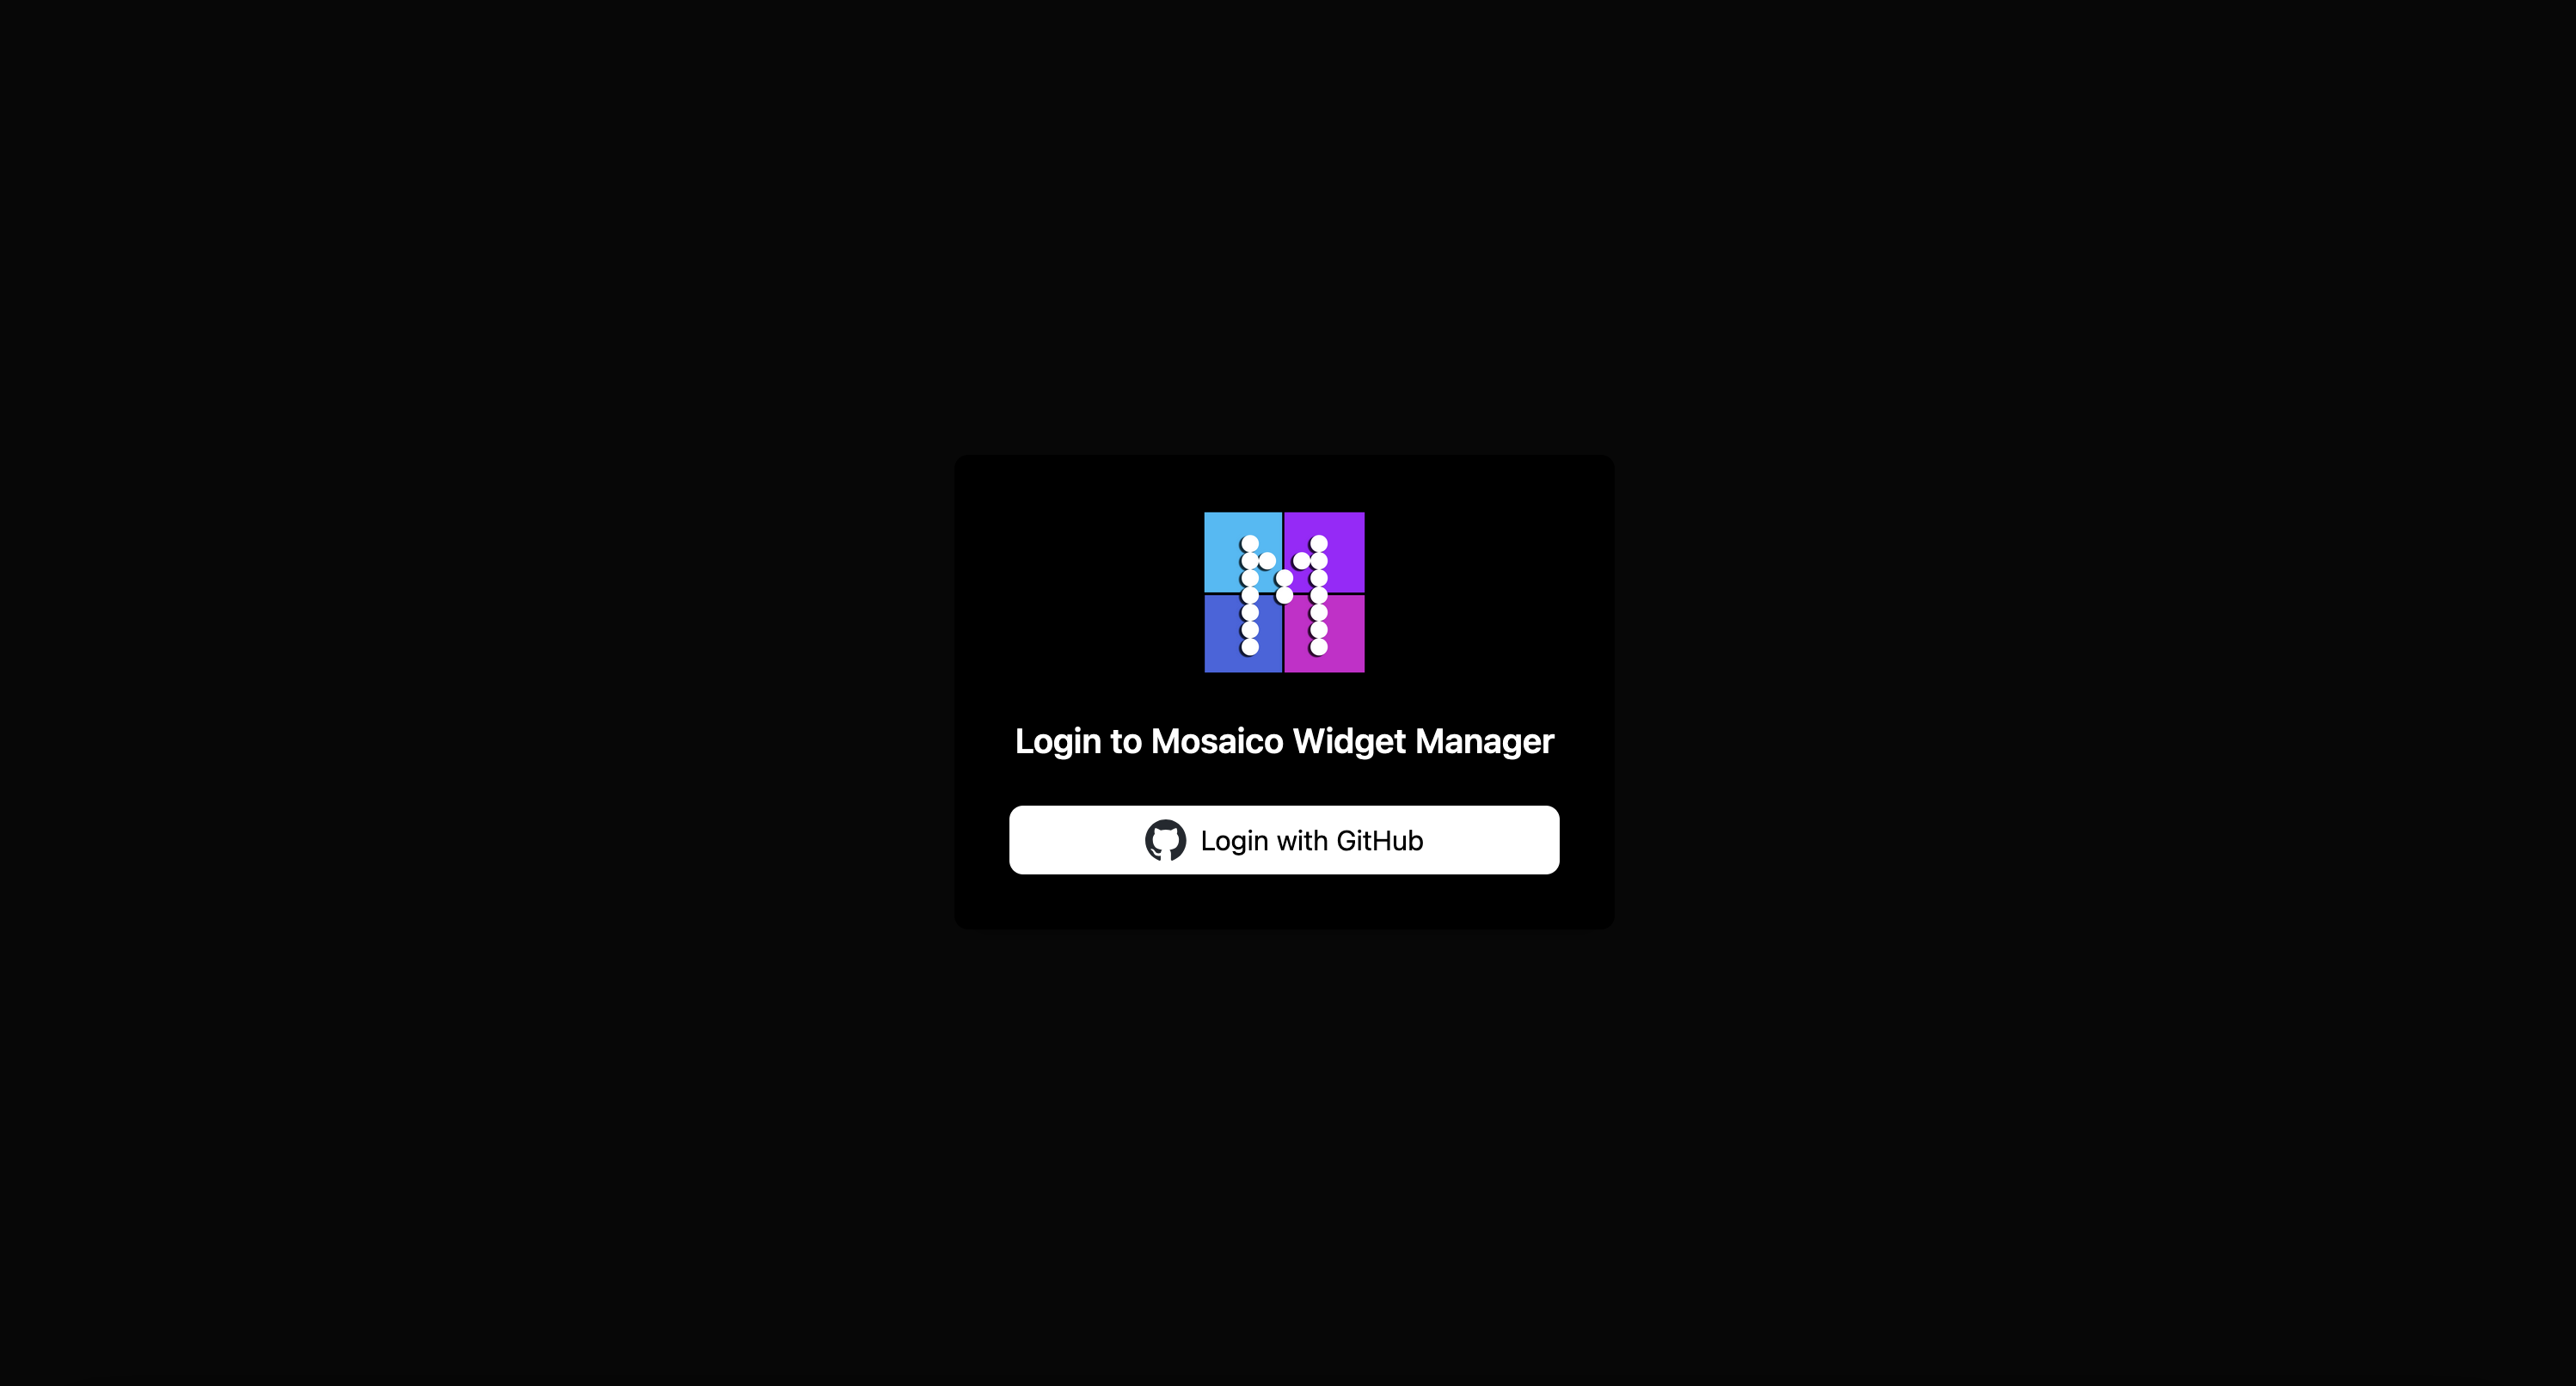
\includegraphics[width=\textwidth]{tesi/img/website_demo/login.png} \caption*{Login with GitHub} \end{minipage} \begin{minipage}[b]{0.49\textwidth} \centering 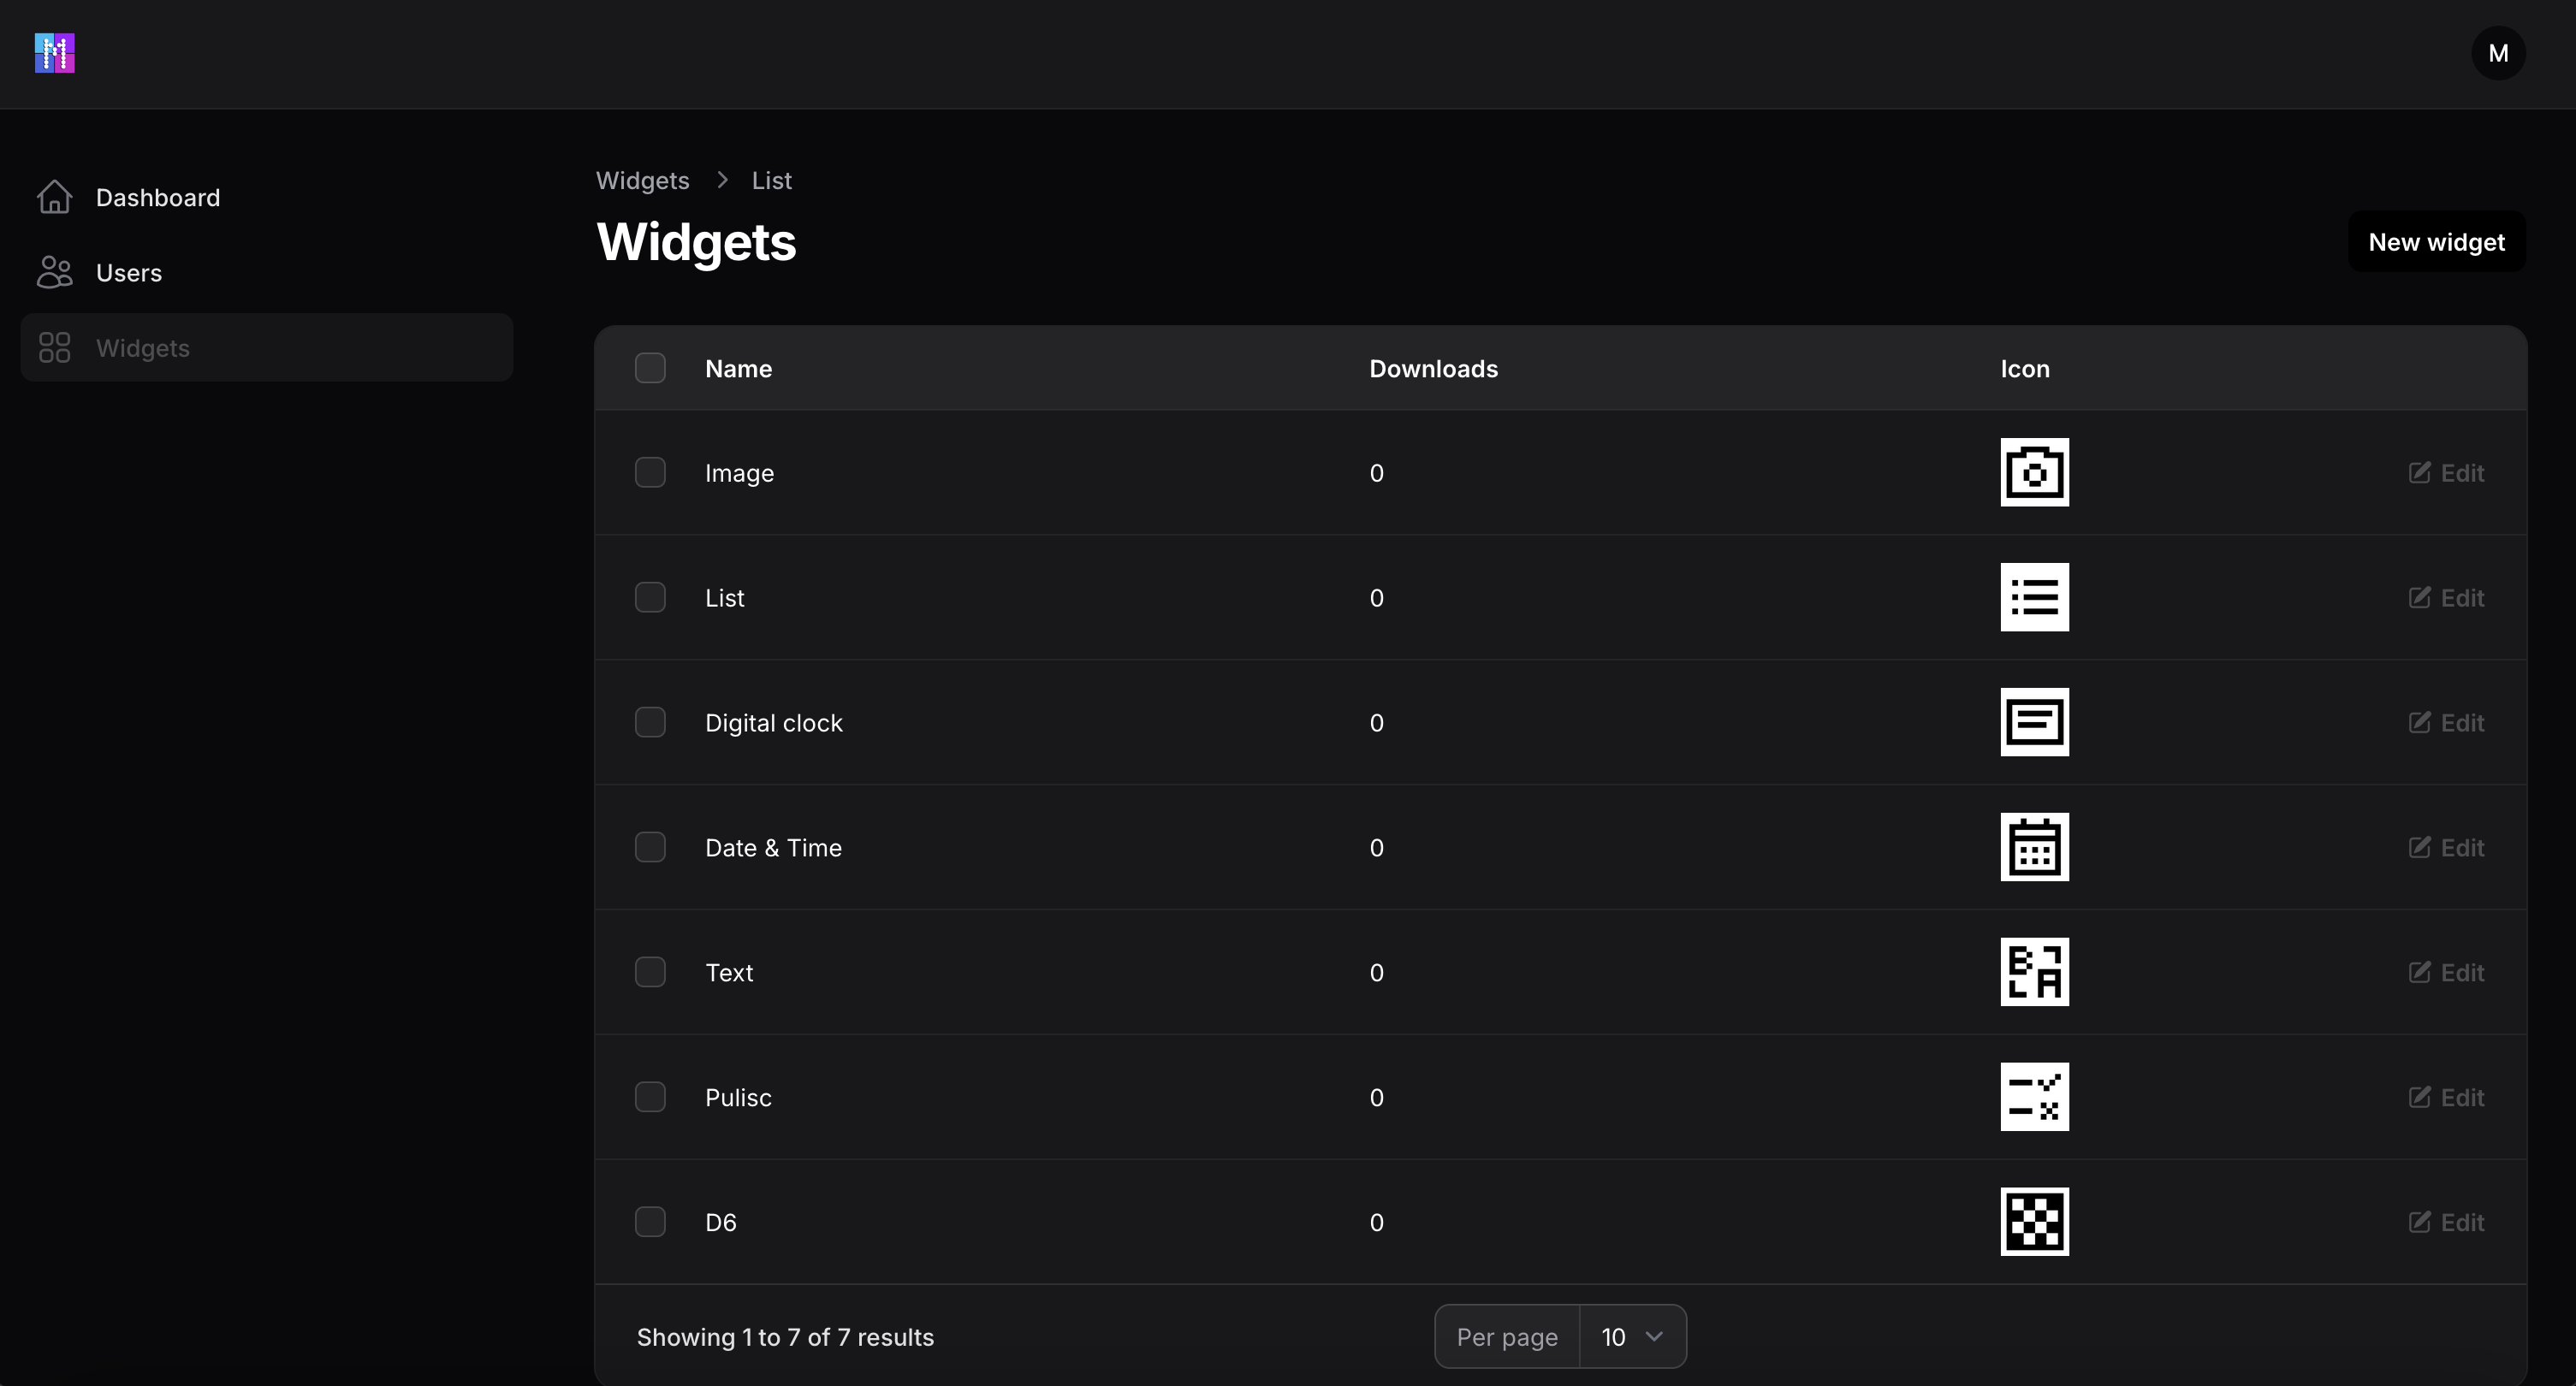
\includegraphics[width=\textwidth]{tesi/img/website_demo/widgets.png} \caption*{Developer's Widgets} \end{minipage} \end{figure}

The user interface has been designed to be intuitive and accessible, ensuring that developers can easily manage their contributions. Developers are required to provide the following information for each widget submission:

\begin{itemize} \item Name of the widget \item An icon representing the widget \item A short tagline or description, displayed beneath the widget’s name \item A comprehensive markdown description, which will appear on the store page \item A series of images, presented in a carousel on the store page \item A link to a valid Git repository, from which the widget can be downloaded \end{itemize}

\begin{figure}[h] \centering \begin{minipage}[b]{0.49\textwidth} \centering 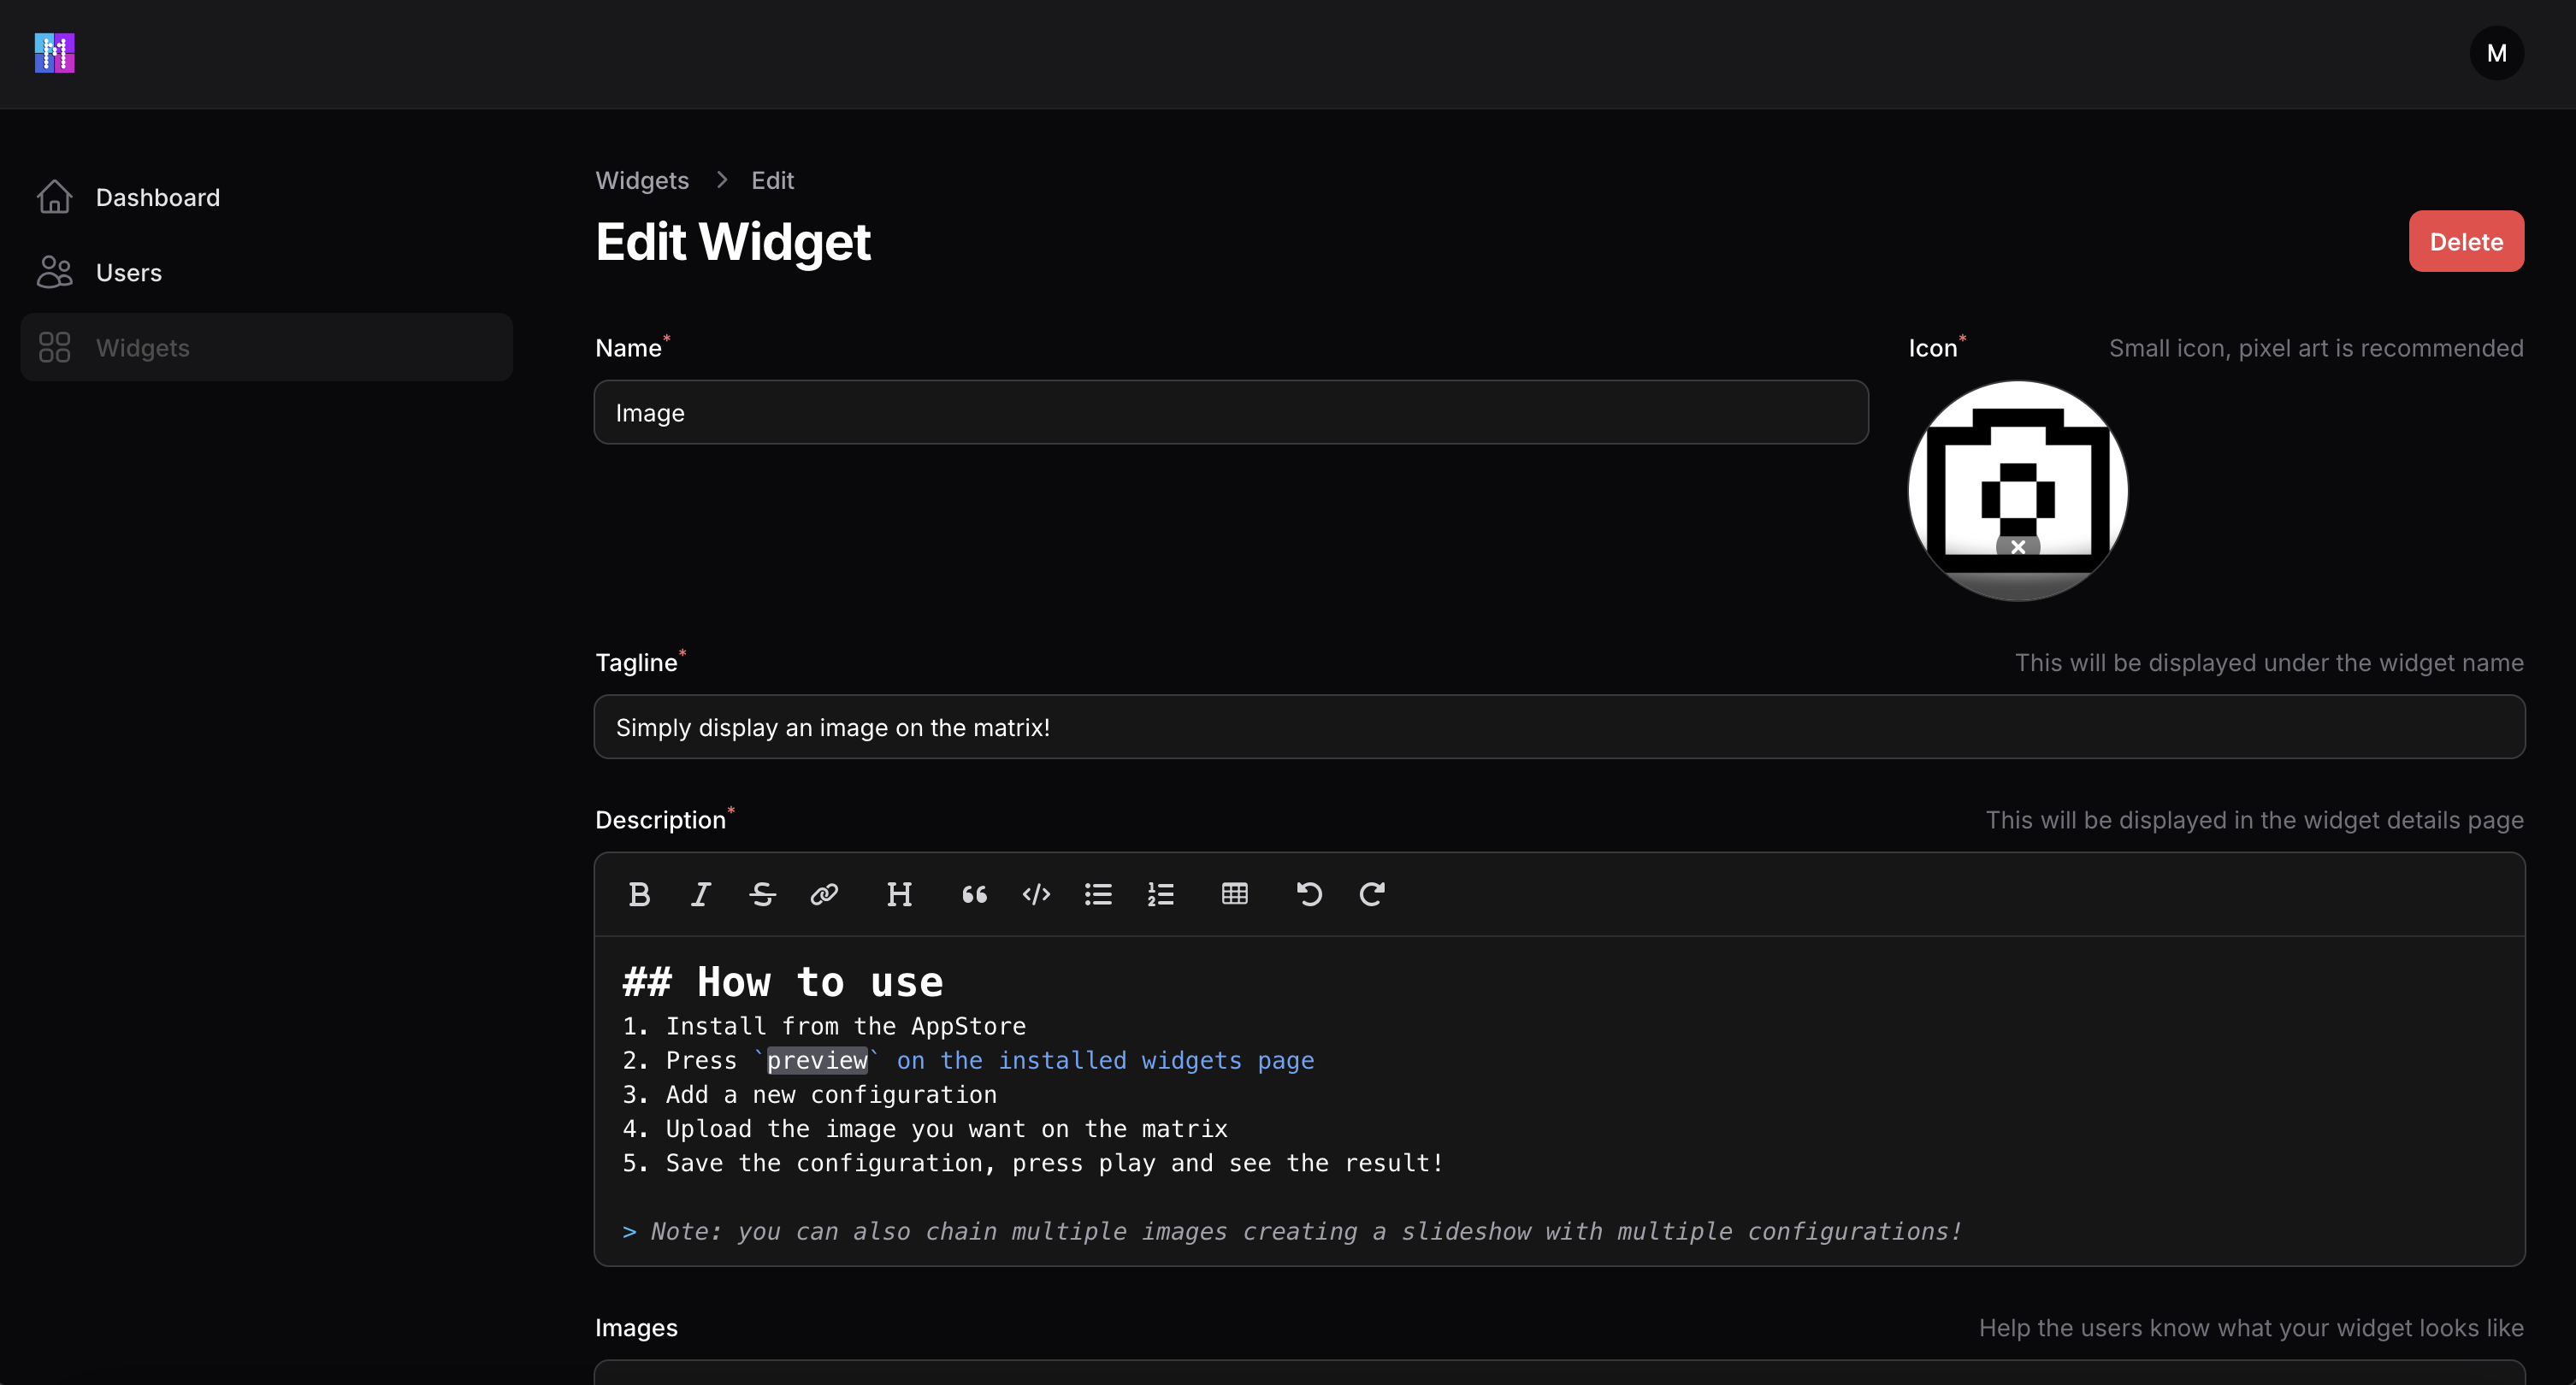
\includegraphics[width=\textwidth]{tesi/img/website_demo/widget-details.png} \caption*{Edit Widget} \end{minipage} \begin{minipage}[b]{0.49\textwidth} \centering 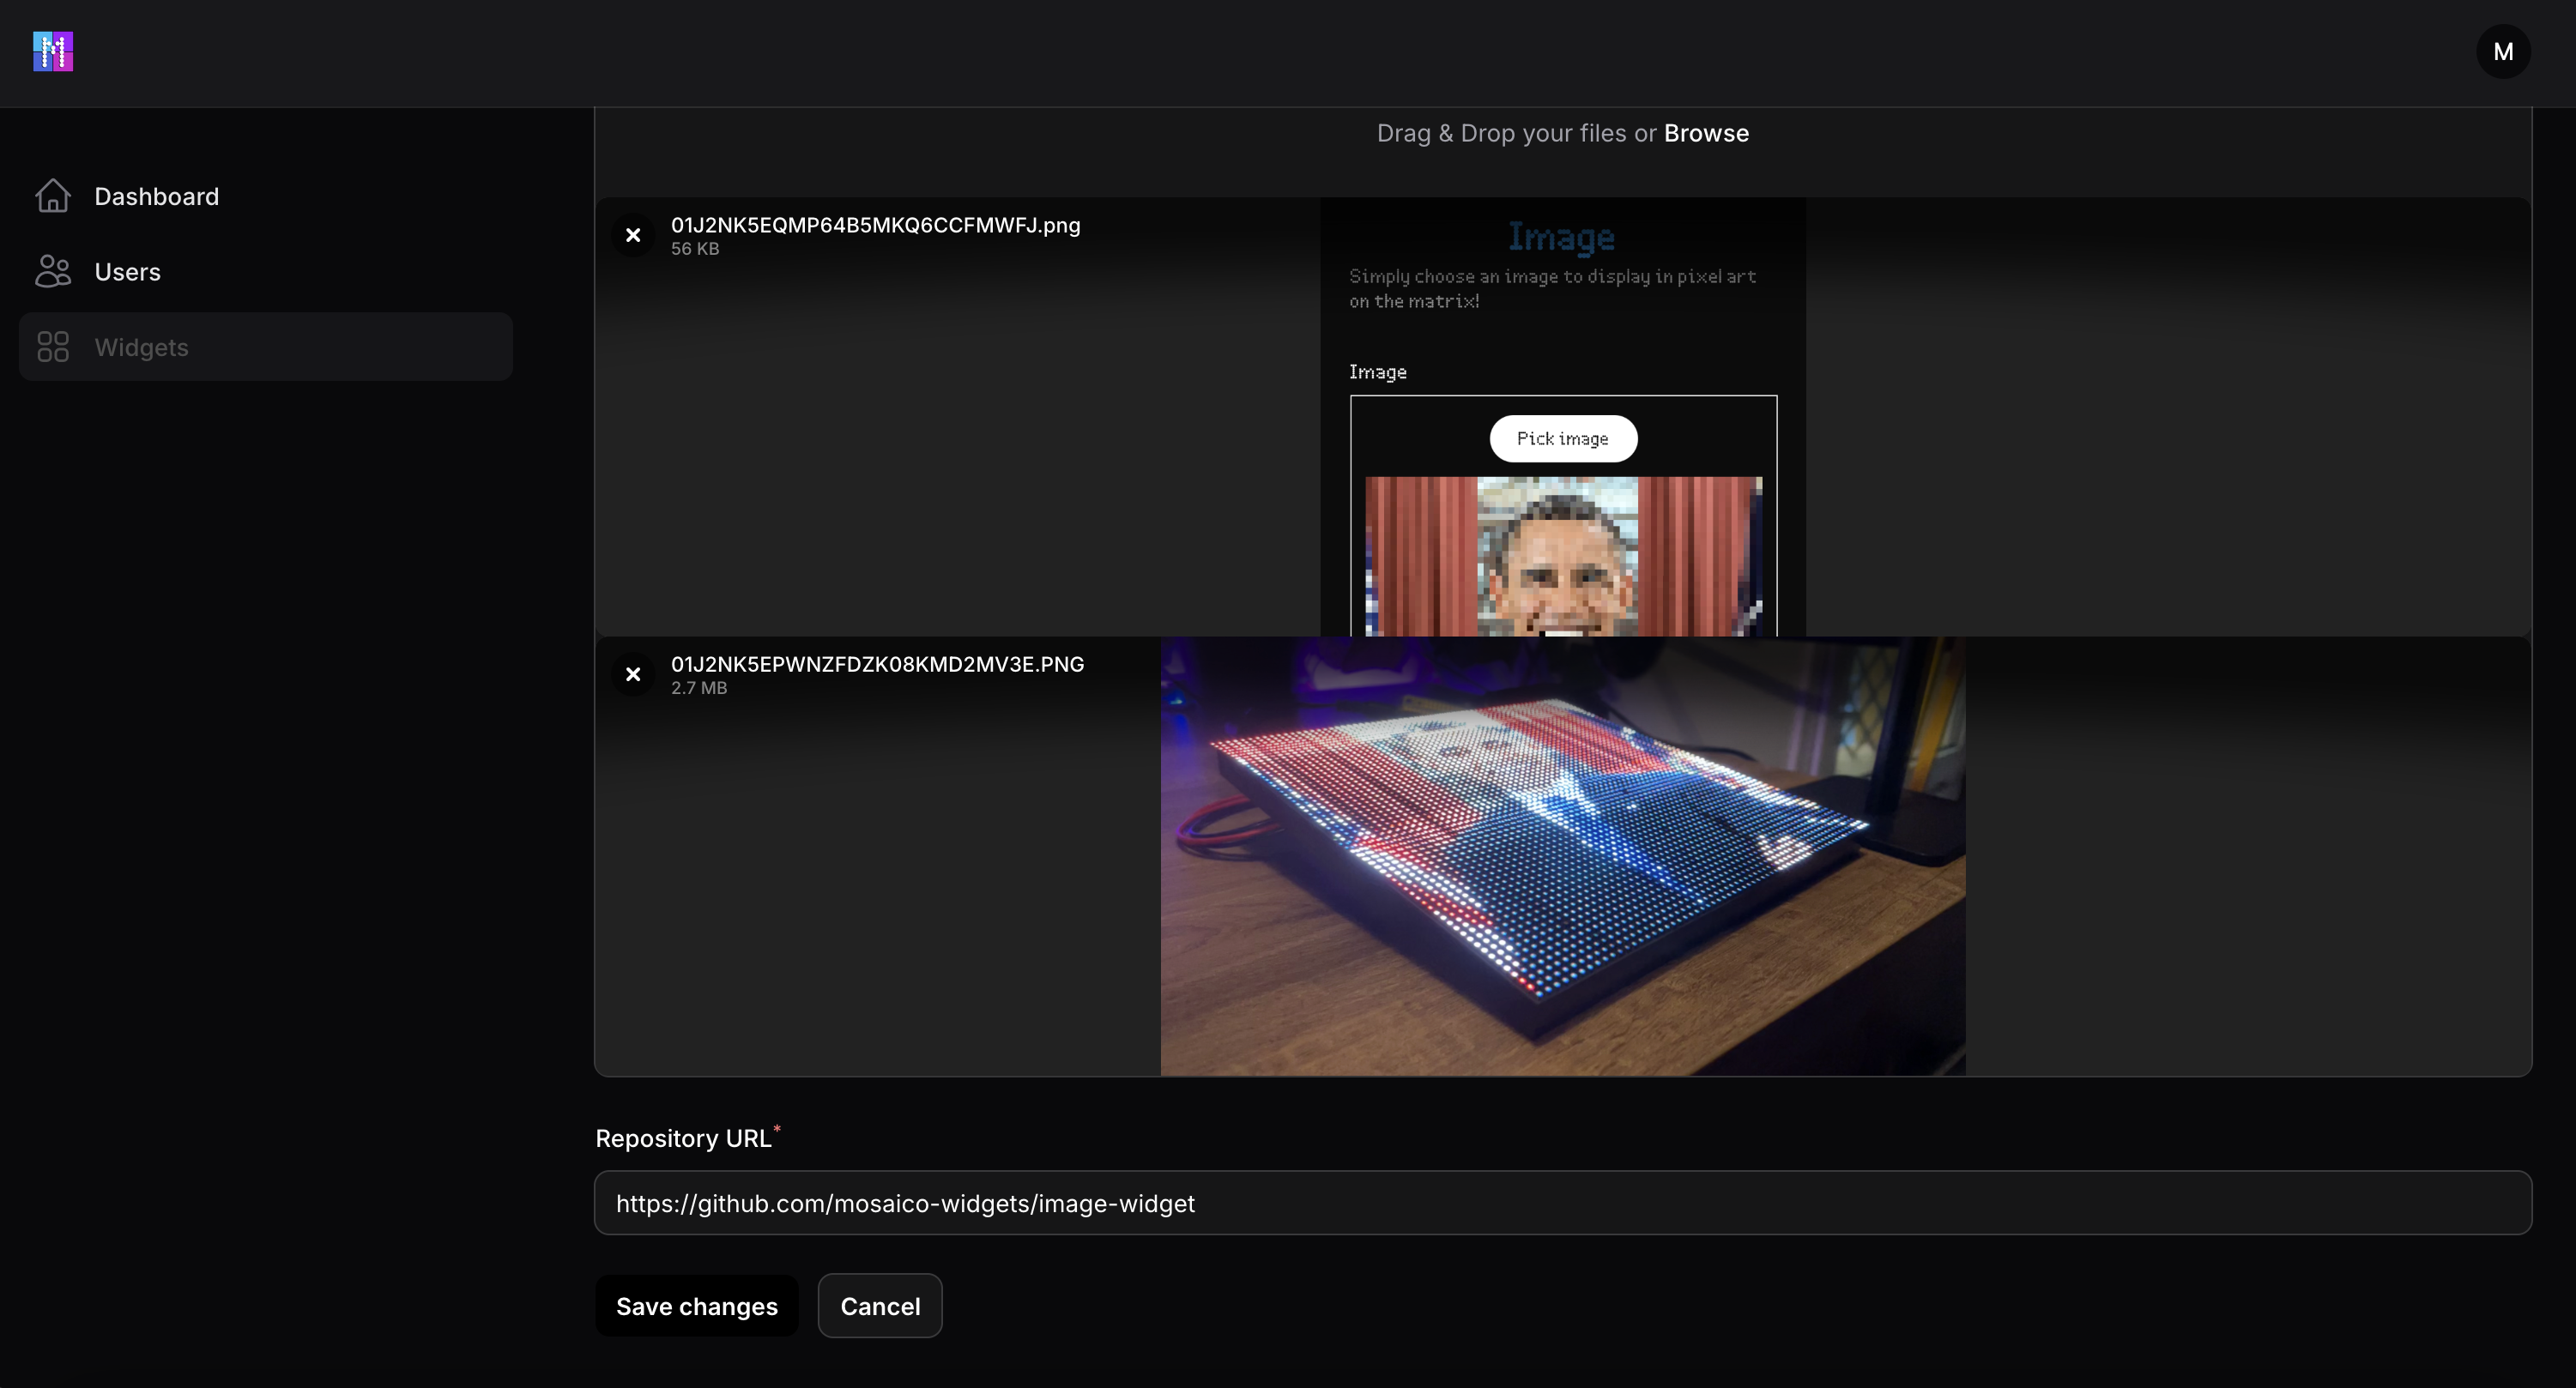
\includegraphics[width=\textwidth]{tesi/img/website_demo/widget-details-2.png} \caption*{Edit Widget - Continued} \end{minipage} \end{figure}

Once all necessary fields have been completed and the developer saves their submission, the widget becomes immediately available to the community.

\section{API}
In the Laravel project, a straightforward REST API is implemented, offering a user-friendly interface for interacting with the Mosaico app store. The API endpoints are designed to be simple and intuitive:

\begin{center} \makebox[\textwidth]{ 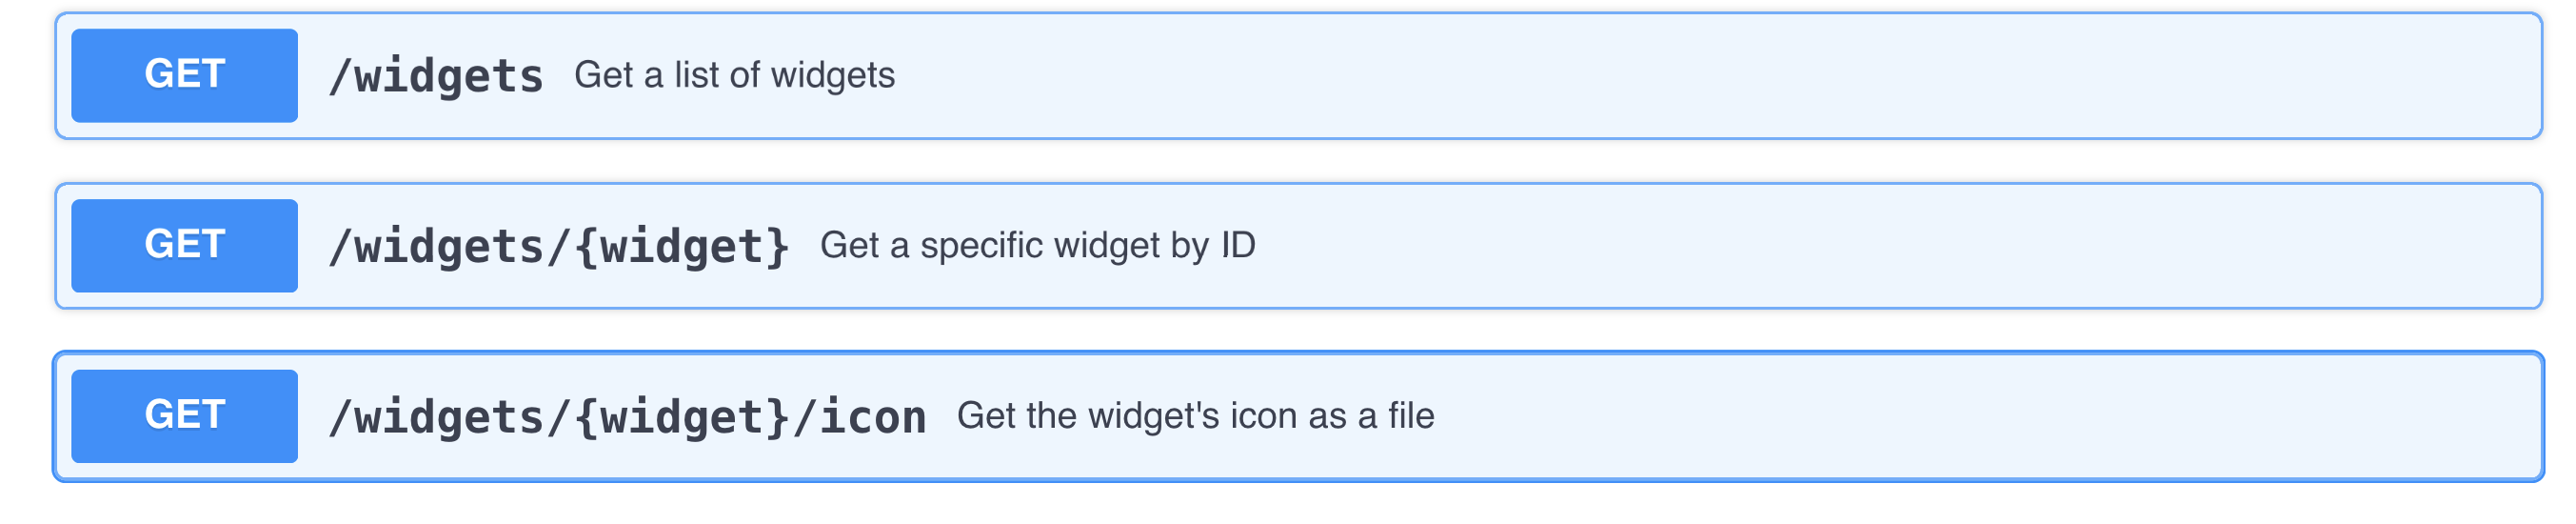
\includegraphics[width=0.8\paperwidth]{tesi/img/website_demo/api.png} } \end{center}

\subsection{Rate Limiter} Given that the only authenticated section of the application is the developer's dashboard, the API remains open for public access, allowing users to browse and utilize its features. However, this accessibility introduces potential vulnerabilities, such as Distributed Denial of Service (DDoS) attacks or spam requests. To mitigate these risks and protect the application’s logic as well as its database from excessive strain, a rate limiting mechanism has been implemented. This mechanism restricts the number of incoming requests from a specific IP address, effectively blocking those that exhibit suspicious behavior.
\newpage
\section{Landing Page}
A well-designed and visually appealing landing page is crucial as the introductory interface for my project. To achieve this, I focused on creating a catchy, minimalistic, and attractive design that effectively captures the essence of Mosaico while ensuring user engagement. The aesthetic appeal of the landing page not only draws users in but also facilitates intuitive navigation, enabling visitors to quickly locate the information and features they seek.

The website can be accessed at \url{https://mosaico.murkrowdev.org}. From this central hub, users can explore all the web-based functionalities of the application. This includes access to the developer dashboard, which allows for seamless interaction with the platform's development tools, as well as links to the project's GitHub repository, where users can contribute to or modify the source code. Additionally, comprehensive documentation is provided, guiding users through the various features and capabilities of Mosaico. This multi-faceted approach ensures that users have all the necessary resources at their fingertips, fostering an environment of collaboration and innovation within the community.

\begin{figure}[H]
\centering
\begin{minipage}[b]{0.49\textwidth}
\centering
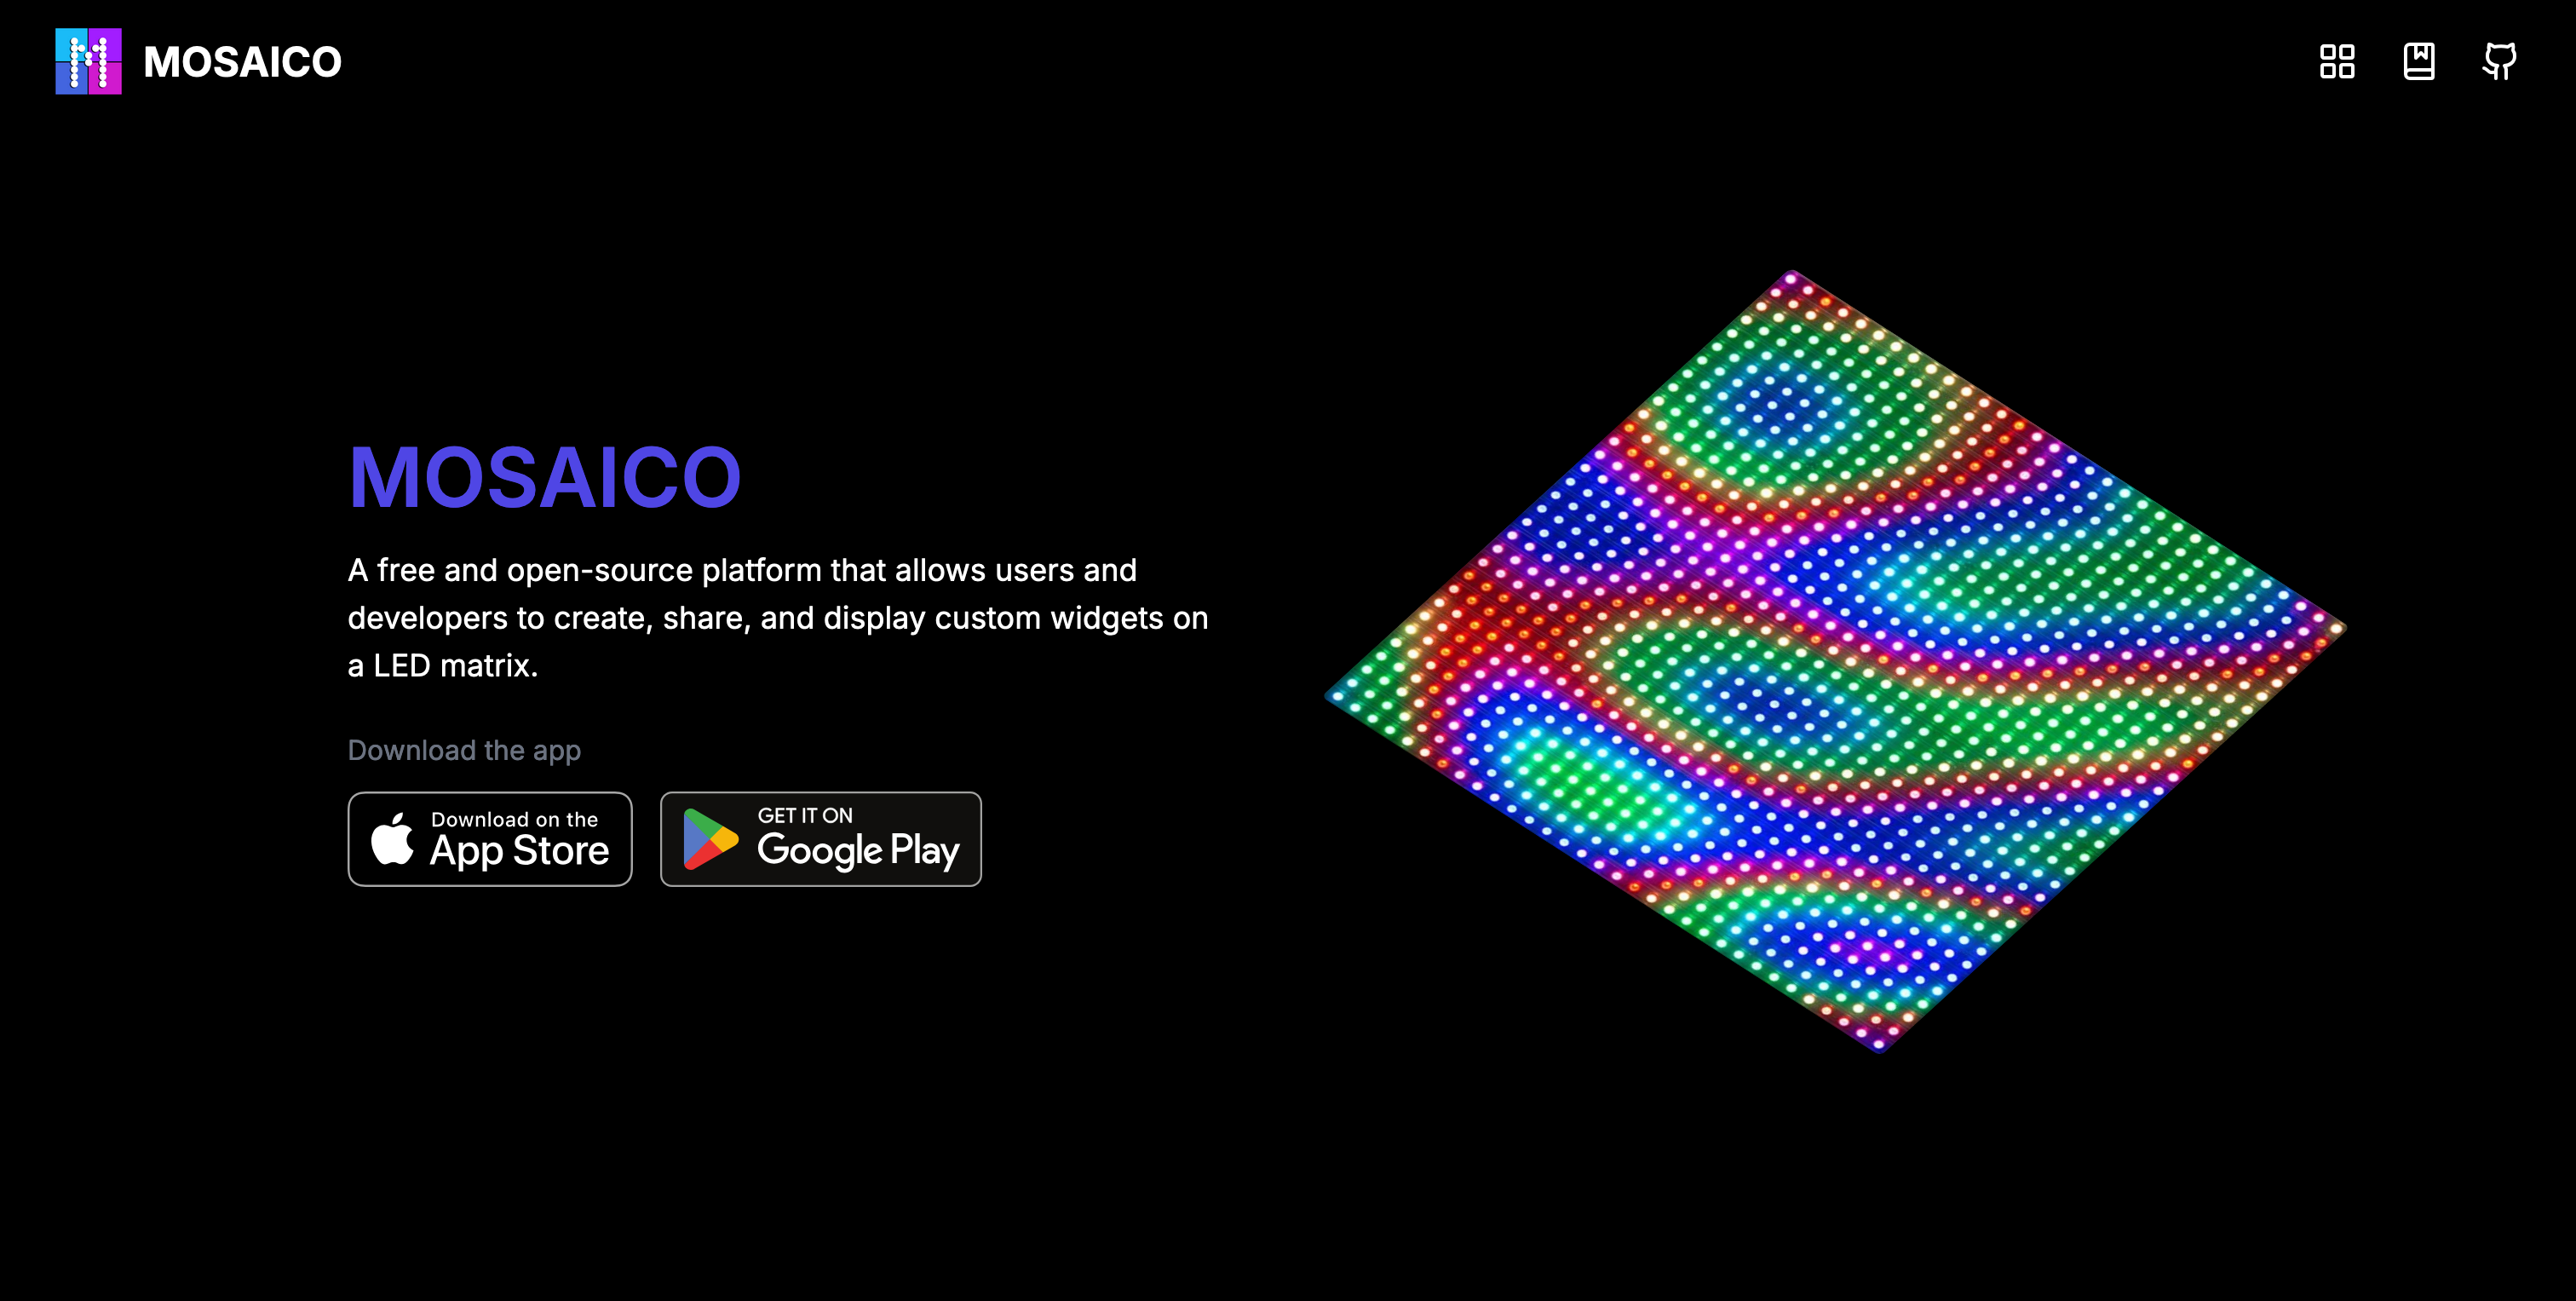
\includegraphics[width=\textwidth]{tesi/img/website_demo/landing/1.png}
\caption*{Call to action}
\end{minipage}
\begin{minipage}[b]{0.49\textwidth}
\centering
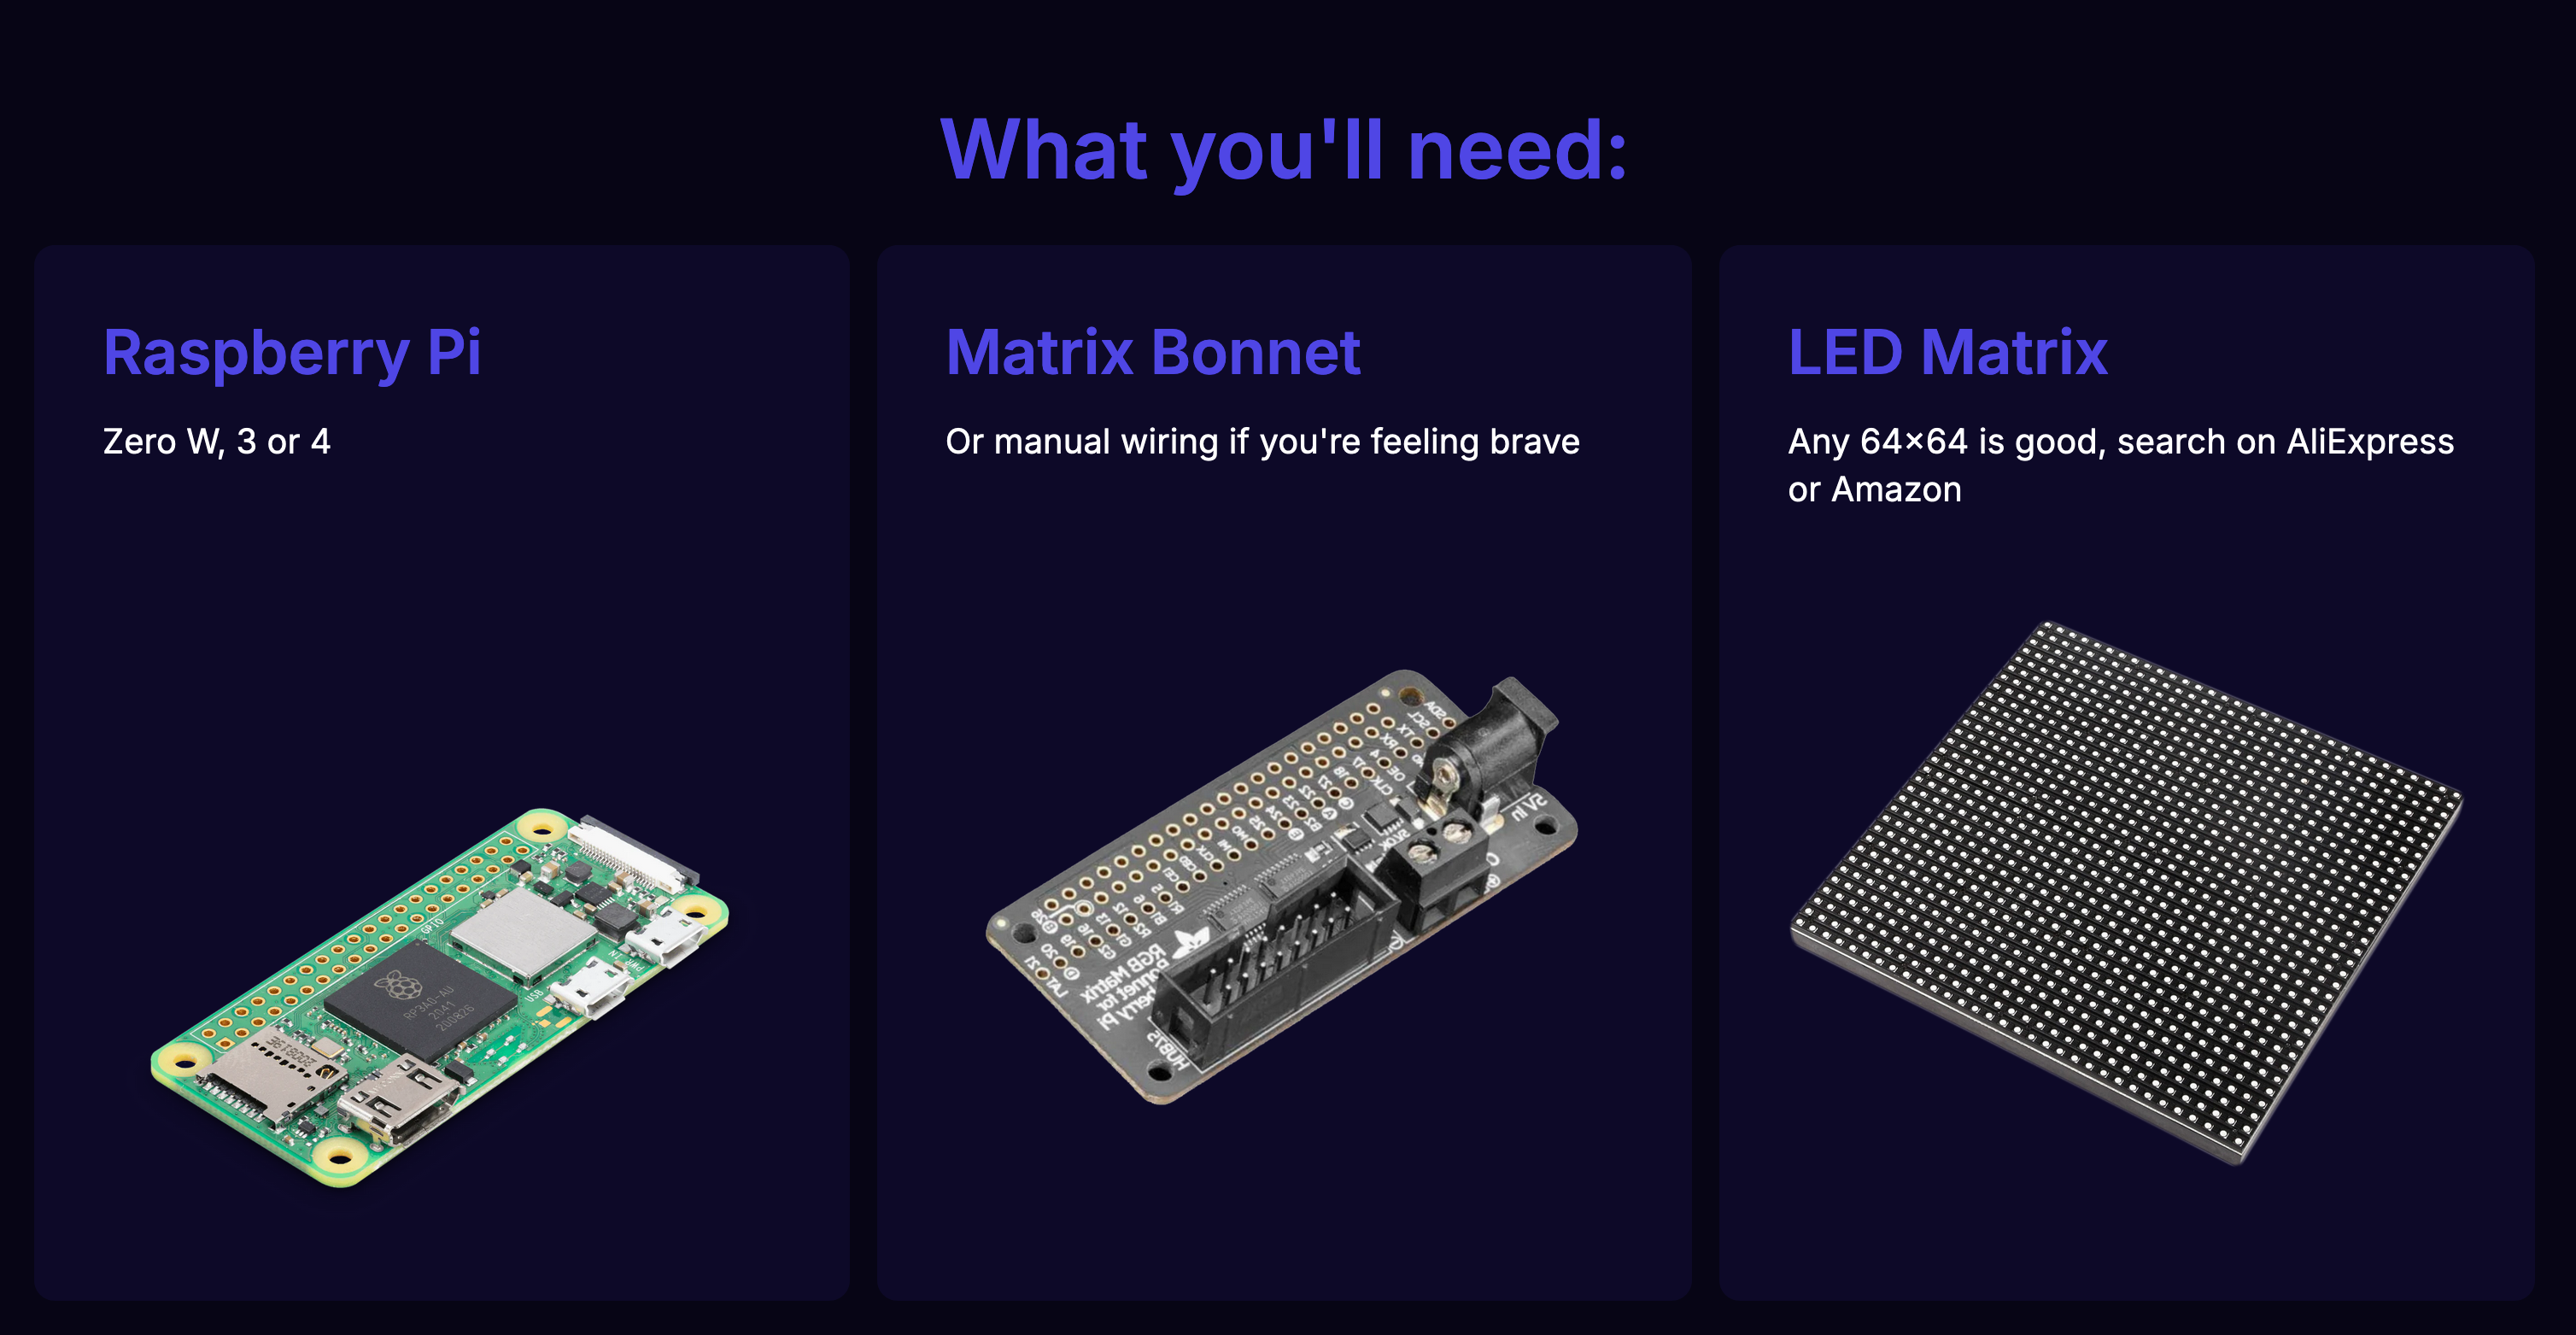
\includegraphics[width=\textwidth]{tesi/img/website_demo/landing/2.png}
\caption*{Hardware components}
\end{minipage}
\end{figure}

\begin{figure}[H]
\centering
\begin{minipage}[b]{0.49\textwidth}
\centering
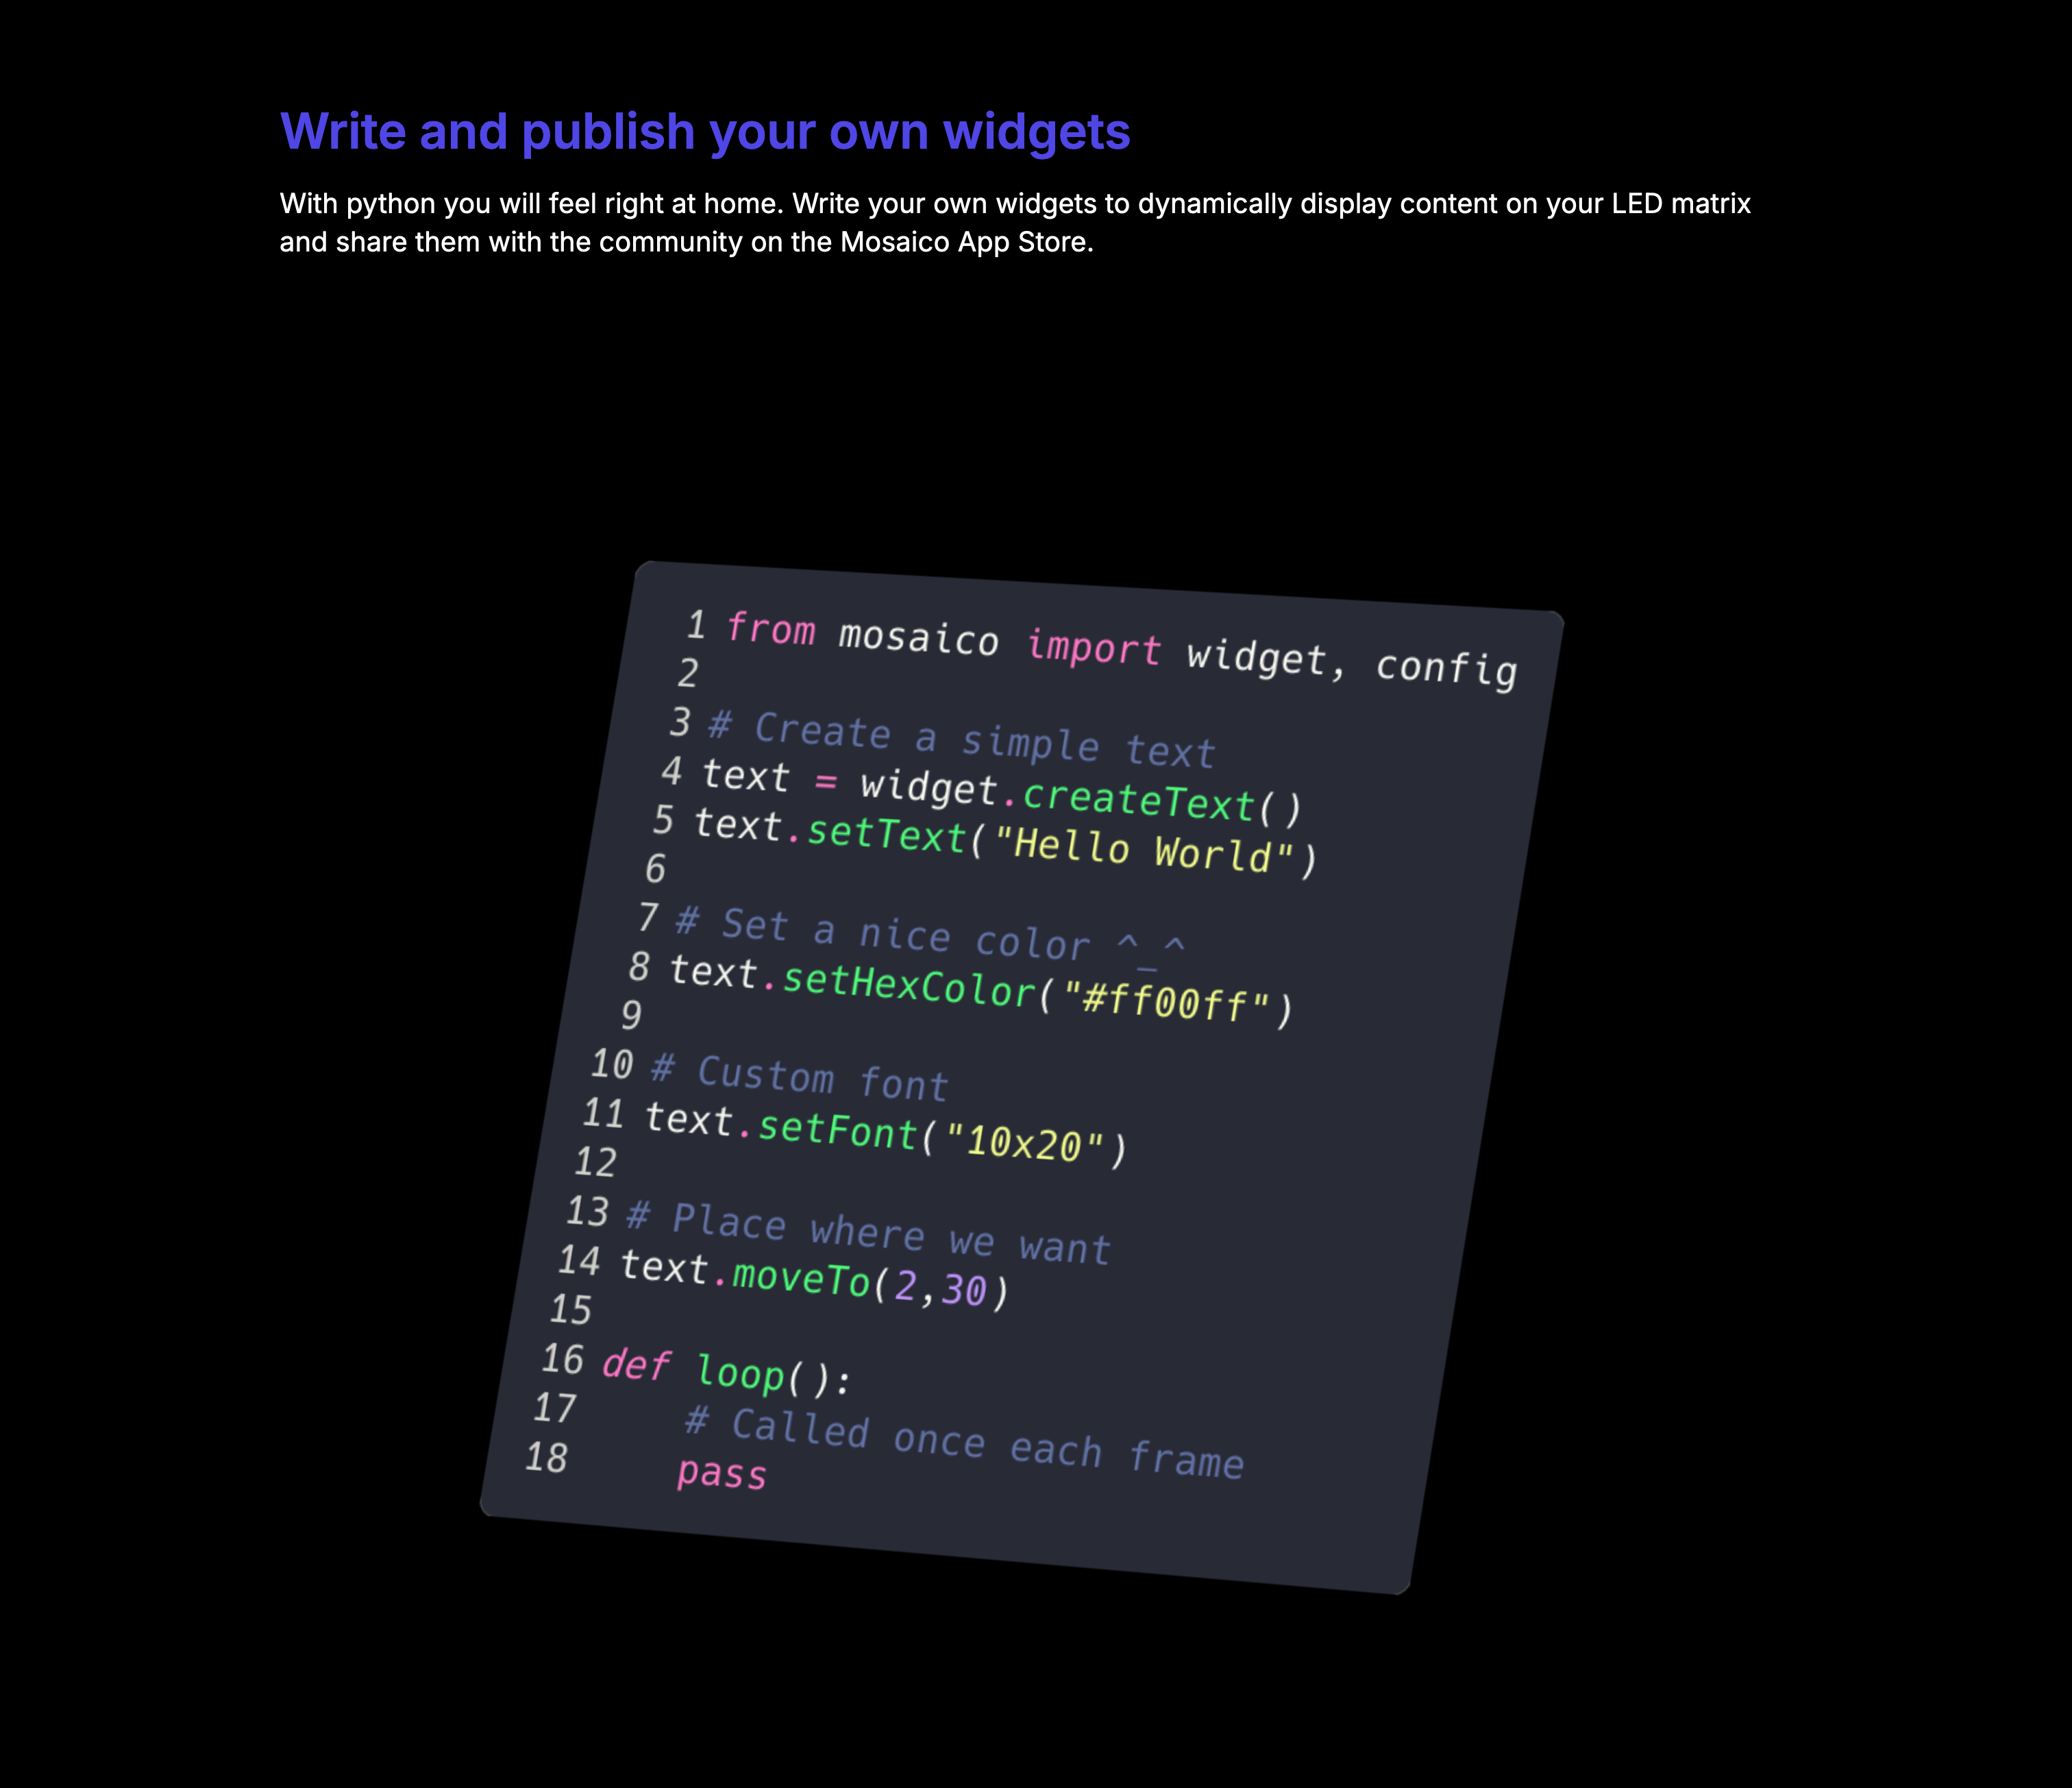
\includegraphics[width=\textwidth]{tesi/img/website_demo/landing/3.png}
\caption*{Widgets}
\end{minipage}
\begin{minipage}[b]{0.49\textwidth}
\centering
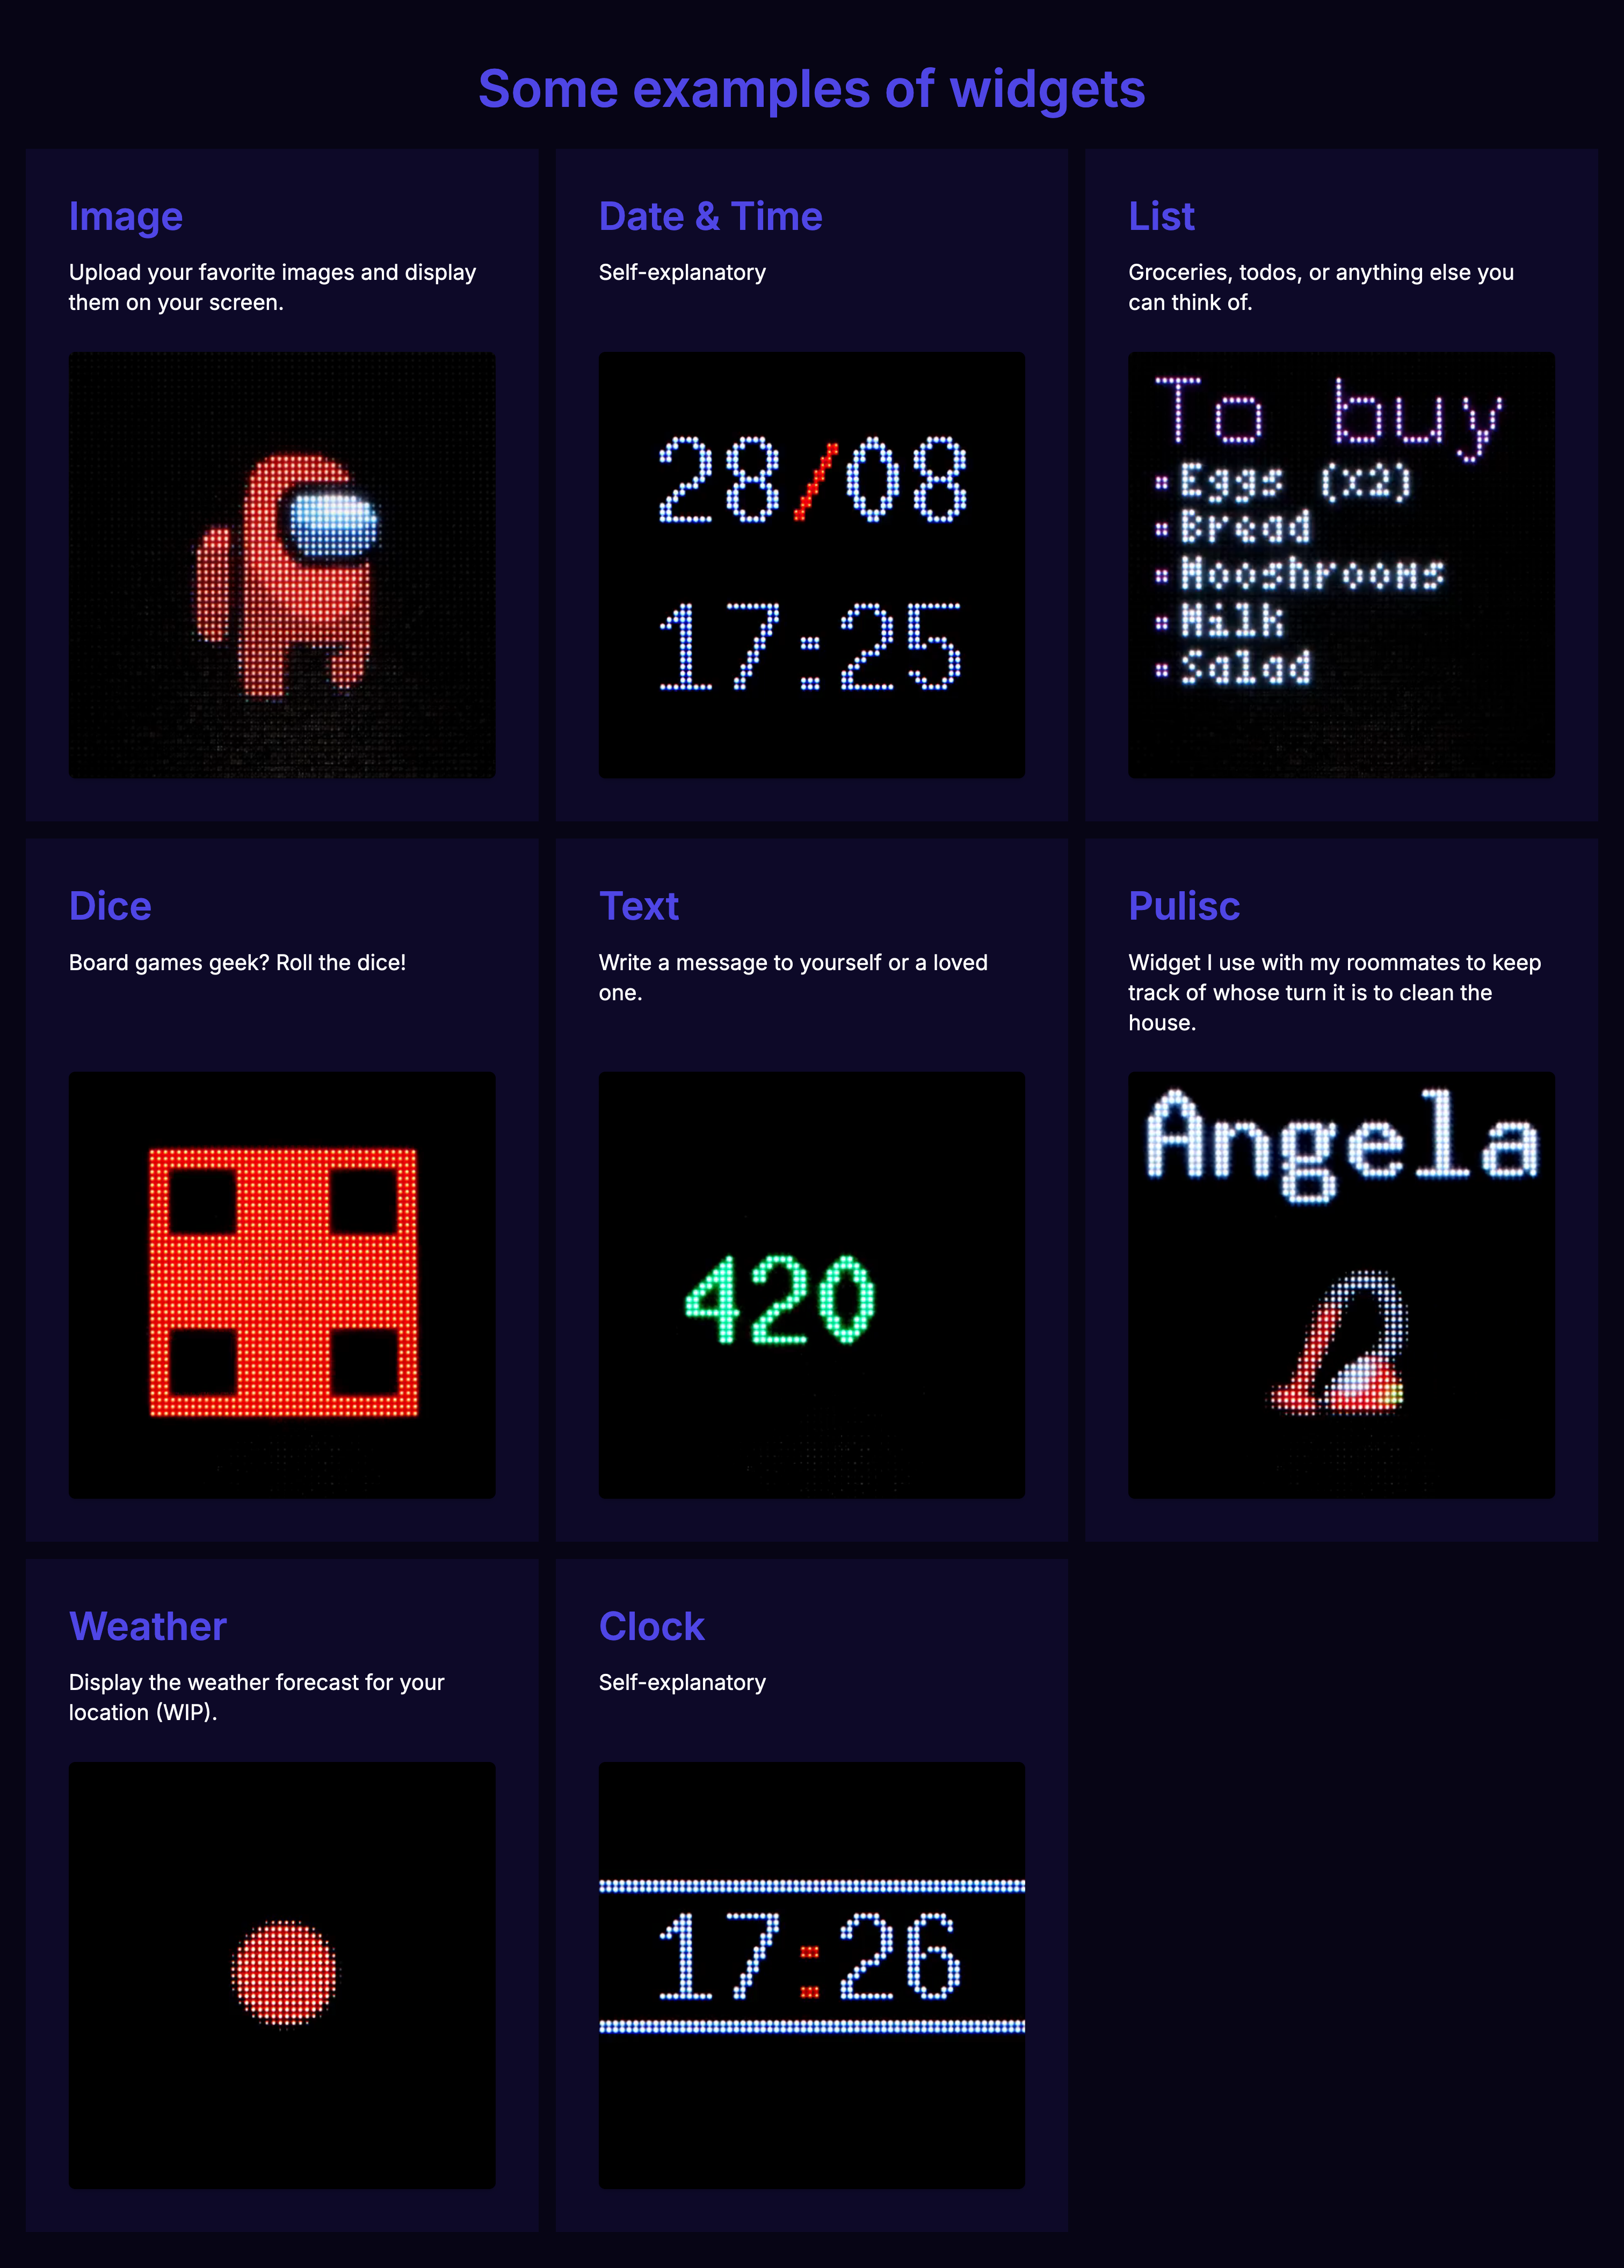
\includegraphics[width=\textwidth]{tesi/img/website_demo/landing/4.png}
\caption*{Widgets showcase}
\end{minipage}
\end{figure}

\begin{figure}[H]
\centering
\begin{minipage}[b]{0.49\textwidth}
\centering
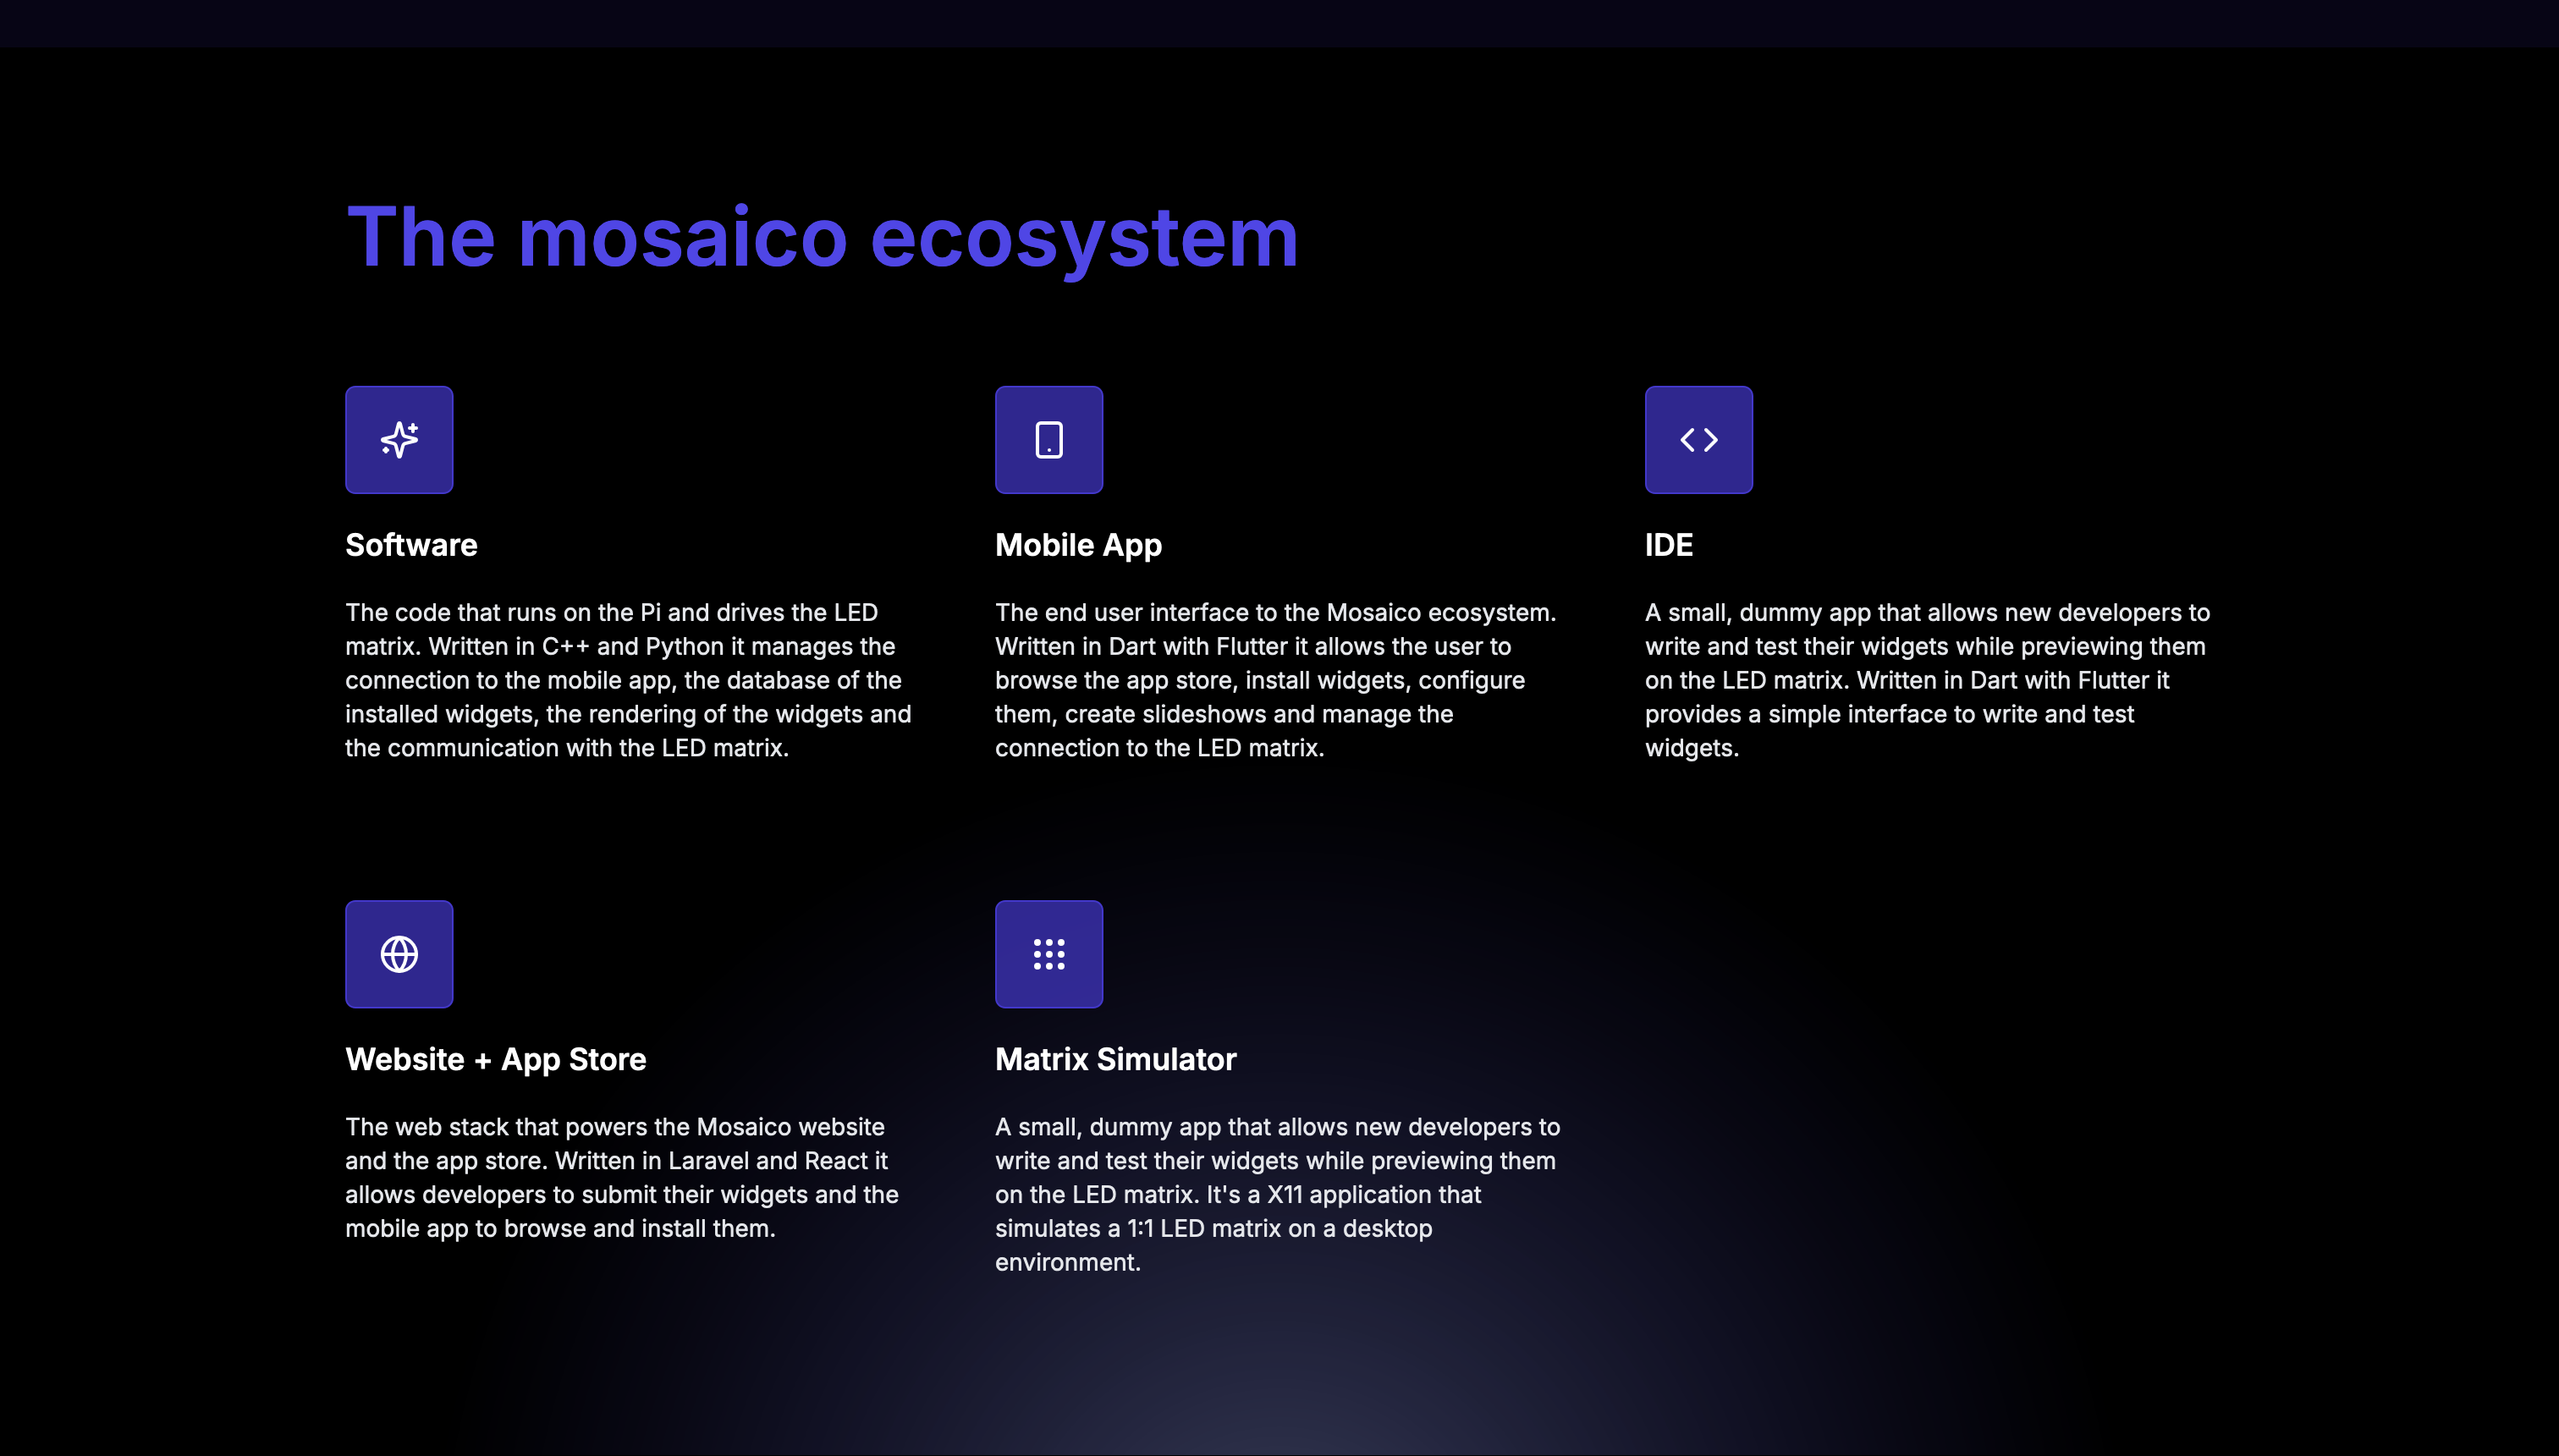
\includegraphics[width=\textwidth]{tesi/img/website_demo/landing/5.png}
\caption*{The ecosystem}
\end{minipage}
\begin{minipage}[b]{0.49\textwidth}
\centering
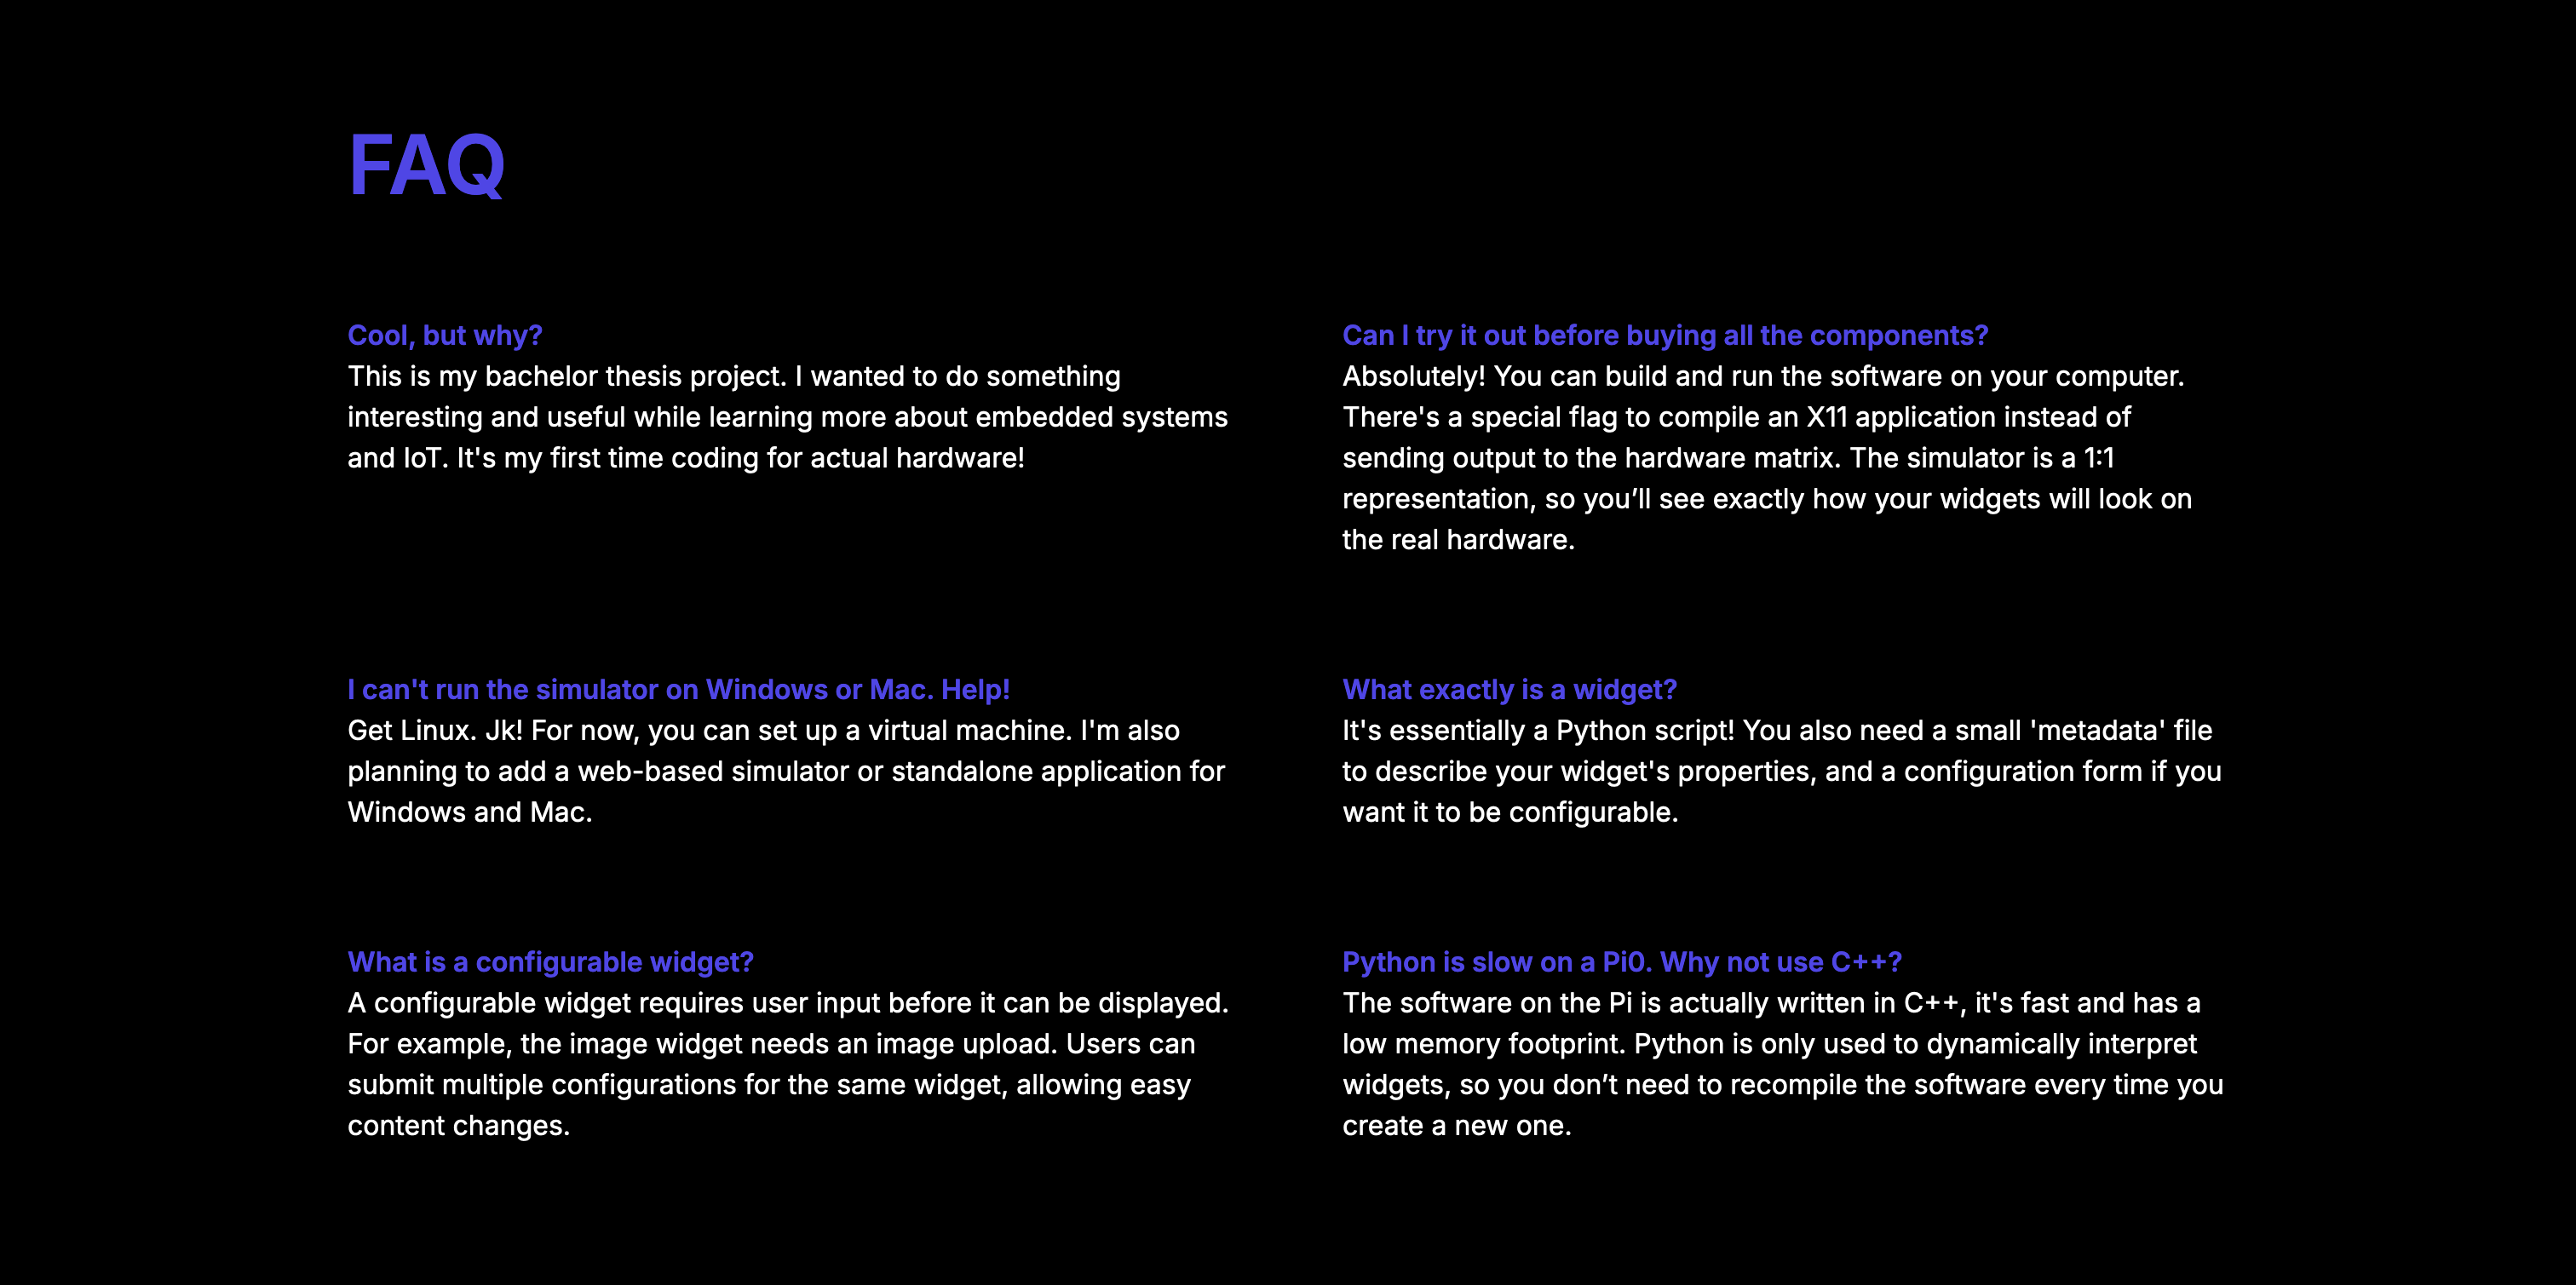
\includegraphics[width=\textwidth]{tesi/img/website_demo/landing/6.png}
\caption*{FAQ}
\end{minipage}
\end{figure}

\newpage
\section{Documentation}
When developing an open-source project, the importance of well-structured and comprehensive documentation cannot be overstated. Effective documentation serves as a vital resource for users and developers alike, providing essential guidance and facilitating engagement with the project. For this purpose, I utilized MkDocs\footnote{\url{https://www.mkdocs.org/}}, a powerful static site generator that enables the creation of documentation using Markdown. This tool allows for the automatic generation of a well-formatted and organized static HTML website, which is readily deployable within my main Laravel project.

The documentation is accessible at the following URL: \url{https://mosaico.murkrowdev.org/docs}. It provides a general overview of the Mosaico project, outlining its objectives and features. However, the primary focus of the documentation is directed towards widget developers aspiring to create and publish widgets in the app store. By offering detailed instructions, examples, and best practices, the documentation aims to empower developers to effectively engage with the Mosaico ecosystem, fostering creativity and collaboration within the community.